\documentclass{article}

% Language setting
% Replace `english' with e.g. `spanish' to change the document language
\usepackage[english]{babel}

% Set page size and margins
% Replace `letterpaper' with `a4paper' for UK/EU standard size
\usepackage[letterpaper,top=2cm,bottom=2cm,left=3cm,right=3cm,marginparwidth=1.75cm]{geometry}

% Useful packages
\usepackage{amsmath,amssymb,amsthm}
\usepackage{amsfonts}
\usepackage{graphicx}
\usepackage{float} 
\usepackage[colorlinks=true, allcolors=blue]{hyperref}
\usepackage{fancyhdr} % Header/footer customization
\usepackage{tcolorbox} % For definition/theorem boxes
\usepackage{enumitem} % For custom lists
\usepackage{booktabs} % For textbook look
\usepackage{tikz}
\usetikzlibrary{shapes, positioning, arrows.meta, calc}

% --- amsthm theorem styles ---

% plain style: boldface title, italicized body
\theoremstyle{plain}
\newtheorem{theorem}{Theorem}[section]
\newtheorem{lemma}[theorem]{Lemma}
\newtheorem{corollary}[theorem]{Corollary}
\newtheorem{proposition}[theorem]{Proposition}
\newtheorem{conjecture}[theorem]{Conjecture}

% definition style: boldface title, Roman body
\theoremstyle{definition}
\newtheorem*{definition}{Definition}
\newtheorem*{condition}{Condition}
\newtheorem*{problem}{Problem}
\newtheorem*{example}{Example}

% remark style: italicized title, Roman body
\theoremstyle{remark}
\newtheorem*{remark}{Remark}
\newtheorem*{note}{Note}
\newtheorem{annotation}{Annotation}
\newtheorem{claim}{Claim}
\newtheorem{case}{Case}
\newtheorem{acknowledgment}{Acknowledgment}
\newtheorem{conclusion}{Conclusion}

\title{CS1231S: Discrete Structures

(Notes \&\ Extras)

Version 1.0}
\author{Ang Wei Jian}
\date{\today}

\begin{document}
\maketitle \newpage

\tableofcontents \newpage

\section{Speaking Mathematically}
To start off your discrete math journey, you will have to know \textbf{AND} get comfortable with math symbols!

\subsection{Mathematical Symbols}

\begin{table}[H]
    \centering
    \begin{tabular}{ll}
        \toprule
        \textbf{Symbol} & \textbf{Definition} \\
        \midrule
        $\forall$ & for all \\
        $\exists$ & there exists \\
        $\exists!$ & there exists a unique \\
        $\mathbb{N}$ & the set of all natural numbers $\{0,1,2,3, \dots\}$ \\
        $\mathbb{Z}$ & the set of all integers \textbf{(For CS1231S: Includes 0)} \\
        $\mathbb{Q}$ & the set of all rational numbers \\
        $\mathbb{R}$ & the set of all real numbers \\
        $\mathbb{Z}^{+/-}$ & the set of all positive/negative integers \\
        $\mathbb{Z}_{\geq i}$ & the set of all integers $\geq i$ \\
        $\mathbb{Z}_n$ & the set of integers from 1 to $n$ $\{1,2, \dots, n\}$ \\
        \bottomrule
    \end{tabular}
    \caption{Mathematical Symbols}
    \label{tab:symbols}
\end{table}

\subsection{Mathematical Statements}

\begin{table}[H]
    \centering
    \begin{tabular}{ll}
        \toprule
        \textbf{Definition} & \textbf{Symbol} \\
        \midrule
        Universal Statements & $\forall$ \\
        Existential Statements & $\exists$ \\
        Conditional Statements & `if $p$ then $q$' ($p \Rightarrow q$) \\
        Universal Conditional Statements & $\forall x, P(x) \Rightarrow Q(x)$ \\
        Universal Existential Statements & $\forall x \exists y, \dots$ \\
        Existential Universal Statements & $\exists x \forall y, \dots$ \\
        \bottomrule
    \end{tabular}
    \caption{Mathematical Statements}
    \label{tab:statements}
\end{table}

\newpage

\section{Logic of Compound Statements}

\subsection{Statements}

\begin{definition}[Statement]
A statement is either true or false, but not both.
\end{definition}

\begin{table}[H]
    \centering
    \begin{tabular}{ll} 
        \toprule
        \textbf{Law/Statement} & \textbf{Symbols} \\ 
        \midrule 
        Negation & $\neg p$ \\ 
        Conjunction & $p \wedge q$ \\ 
        Disjunction & $p \vee q$ \\ 
        Logical Equivalence & $p \equiv q$ \\ 
        Tautology & $\top$ (true) \\ 
        Contradiction & $\bot$ (false) \\ 
        Conditional & $p \Rightarrow q$, ``if $p$, then $q$'' \\ 
        Contrapositive & $\neg q \Rightarrow \neg p$, ``if not $q$, then not $p$'' \\ 
        Converse & $q \Rightarrow p$, ``if $q$, then $p$'' \\ 
        Inverse & $\neg p \Rightarrow \neg q$, ``if not $p$, then not $q$'' \\ 
        \bottomrule
    \end{tabular}
    \caption{Statements}
    \label{tab:statement}
\end{table}

\subsubsection{Contrapositive, Converse, Inverse}
A conditional is logically equivalent to its contrapositive. Inverses and converses are contrapositives of each other. However, a conditional is \textbf{not} equivalent to its converse or inverse.
\[
    (p \Rightarrow q \equiv \neg q \Rightarrow \neg p) \not\equiv (q \Rightarrow p \equiv \neg p \Rightarrow \neg q)
\]

\subsubsection{Only If}
``$p$ \textbf{only if} $q$'' means ``if not $q$, then not $p$'' or ``$q$ is necessary''.
\[
    \neg q \Rightarrow \neg p \equiv p \Rightarrow q
\]

\subsubsection{If and Only If (iff)}
``$p$ \textbf{if and only if} $q$'' means ``$p$ if $q$'' AND ``$p$ only if $q$''.
\[
    p \Leftrightarrow q \equiv (p \Rightarrow q) \wedge (q \Rightarrow p)
\]

\subsubsection{Order of Operations}
Precedence of logical operators from highest to lowest:
\[
    \neg, \quad (\wedge, \vee), \quad \Rightarrow, \quad \Leftrightarrow
\]

\subsection{Necessary and Sufficient Conditions}

\begin{definition}[Sufficient \& Necessary Conditions]
$r$ is a \textbf{sufficient} condition for $s$:
\[ r \Rightarrow s \]
$r$ is a \textbf{necessary} condition for $s$:
\[ \neg r \Rightarrow \neg s \equiv s \Rightarrow r \]
$r$ is a \textbf{sufficient and necessary} condition for $s$:
\[ r \Leftrightarrow s \] 
\end{definition}

\begin{table}[H]
    \centering
    \begin{tabular}{cc|c|c} 
        \toprule
        $p$ & $q$ & $p \Rightarrow q$ & $p \Leftrightarrow q$ \\ 
        \midrule
        T & T & T & T \\ 
        T & F & F & F \\ 
        F & T & T & F \\ 
        F & F & T & T \\ 
        \bottomrule
    \end{tabular}
    \caption{Implication and Equivalence Truth Tables}
    \label{tab:impliesTT}
\end{table}

\subsection{Theorem 2.1.1 Logical Equivalences}

\textbf{Implication Law} (Not part of the Theorem but important all the same)
\[ p \Rightarrow q \equiv \neg p \vee q \]

\begin{table}[H]
    \centering
    \begin{tabular}{lll}
        \toprule
        \textbf{Laws} & \textbf{\textcolor{blue}{Blue}} & \textbf{\textcolor{red}{Red}} \\
        \midrule
        Commutative Law & $p \wedge q \equiv q \wedge p$ & $p \vee q \equiv q \vee p$ \\
        Associative Law & $(p \wedge q) \wedge r \equiv p \wedge (q \wedge r)$ & $(p \vee q) \vee r \equiv p \vee (q \vee r)$ \\
        Distributive Law & $p \wedge (q \vee r) \equiv (p \wedge q) \vee (p \wedge r)$ & $p \vee (q \wedge r) \equiv (p \vee q) \wedge (p \vee r)$ \\
        Identity Law & $p \wedge \textcolor{blue}{\text{true}} \equiv p$ & $p \vee \textcolor{red}{\text{false}} \equiv p$ \\
        Negation Law & $p \vee \neg p \equiv \textcolor{blue}{\text{true}}$ & $p \wedge \neg p \equiv \textcolor{red}{\text{false}}$ \\
        Double Negation Law & $\neg (\neg p) \equiv p$ & \\
        Idempotent Law & $p \wedge p \equiv p$ & $p \vee p \equiv p$ \\
        Universal Bound Law & $p \vee \textcolor{blue}{\text{true}} \equiv \textcolor{blue}{\text{true}}$ & $p \wedge \textcolor{red}{\text{false}} \equiv \textcolor{red}{\text{false}}$ \\
        De Morgan's Law & $\neg (p \wedge q) \equiv \neg p \vee \neg q$ & $\neg (p \vee q) \equiv \neg p \wedge \neg q$ \\
        Absorption Law & $p \vee (p \wedge q) \equiv p$ & $p \wedge (p \vee q) \equiv p$ \\
        Negation of True \& False & $\neg \textcolor{blue}{\text{true}} \equiv \textcolor{red}{\text{false}}$ & $\neg \textcolor{red}{\text{false}} \equiv \textcolor{blue}{\text{true}}$ \\
        \bottomrule
    \end{tabular}
    \caption{Theorem 2.1.1: Logical Equivalences}
    \label{tab:2.1.1}
\end{table}

\subsection{Arguments}

\begin{definition}[Valid \& Sound Arguments]
Arguments often appear in the form:
\begin{center}
    \begin{minipage}{0.4\linewidth}
        \begin{itemize}
            \item[] Hypothesis/Premise 1
            \item[] Hypothesis/Premise 2
            \item[$\therefore$] Conclusion
        \end{itemize}
    \end{minipage}
\end{center}

A \textbf{valid} argument means that no matter what particular statements are substituted for the statement variables in its premises, if the resulting premises are \textbf{all} true, then the conclusion is true.
This can also be written as:
\[ \text{Premise}_1 \wedge \text{Premise}_2 \wedge \dots \Rightarrow \text{Conclusion} \]

An argument is \textbf{sound} iff it is \textbf{valid} AND all its premises are \textcolor{blue}{\text{true}}.
\end{definition}

\subsubsection{Rules of Inference}

\begin{table}[H]
    \centering
    \begin{tabular}{ll} 
        \toprule
        \textbf{Rule} & \textbf{Form} \\ 
        \midrule 
        Modus Ponens & 
        $\begin{array}{l} 
            p \Rightarrow q \\ 
            p \\ 
            \hline 
            \therefore q 
        \end{array}$ \\ 
        \addlinespace
        Modus Tollens & 
        $\begin{array}{l}
            p \Rightarrow q \\ 
            \neg q \\
            \hline
            \therefore \neg p
        \end{array}$ \\ 
        \addlinespace
        Generalization & 
        $\begin{array}{l} 
            p \\ 
            \hline 
            \therefore p \vee q 
        \end{array}$ 
        \quad \text{or} \quad 
        $\begin{array}{l} 
            q \\ 
            \hline 
            \therefore p \vee q 
        \end{array}$ \\ 
        \addlinespace
        Conjunction & 
        $\begin{array}{l}
            p \\ 
            q \\
            \hline
            \therefore p \wedge q
        \end{array}$ \\ 
        \addlinespace
        Specialization & 
        $\begin{array}{l} 
            p \wedge q \\ 
            \hline 
            \therefore p 
        \end{array}$ 
        \quad \text{or} \quad 
        $\begin{array}{l} 
            p \wedge q \\ 
            \hline 
            \therefore q 
        \end{array}$ \\ 
        \addlinespace
        Elimination & 
        $\begin{array}{l} 
            p \vee q \\ 
            \neg q \\
            \hline
            \therefore p 
        \end{array}$ 
        \quad \text{or} \quad 
        $\begin{array}{l} 
            p \vee q \\ 
            \neg p \\
            \hline
            \therefore q 
        \end{array}$ \\ 
        \addlinespace
        Transitivity & 
        $\begin{array}{l}
            p \Rightarrow q \\ 
            q \Rightarrow r \\
            \hline
            \therefore p \Rightarrow r
        \end{array}$ \\ 
        \addlinespace
        Proof by Division into Cases & 
        $\begin{array}{l}
            p \vee q \\ 
            p \Rightarrow r \\
            q \Rightarrow r \\
            \hline
            \therefore r
        \end{array}$ \\ 
        \addlinespace
        Contradiction Rule & 
        $\begin{array}{l}
            \neg p \Rightarrow \text{false} \\ 
            \hline
            \therefore p
        \end{array}$ \\ 
        \bottomrule
    \end{tabular}
    \caption{Table 2.3.1: Rules of Inference}
    \label{tab:2.3.1}
\end{table}

\newpage
\section{Logic of Quantified Statements}
\subsection{Quantified Statements}

\begin{definition}[Predicate]
A \textbf{predicate} $P(x)$ becomes a statement when specific values are substituted for the variable $x$. A \textbf{domain} is the set of values that may be substituted into the variable.
\end{definition}

\begin{definition}[Truth Set]
If $P(x)$ is a predicate and $x$ has domain $D$, the \textbf{truth set} is the subset of $D$ that makes $P(x)$ true when substituted for $x$. Denoted as:
\[ \{x \in D : P(x)\} \]
\end{definition}

\subsubsection{Universal Statement}
\begin{definition}[Universal Statement]
Appears in the form:
\[ \forall x \in D, Q(x) \]
\begin{itemize}
    \item \textcolor{blue}{\text{true}} iff $Q(x)$ is \textcolor{blue}{\text{true}} for \textbf{EVERY} $x \in D$.
    \item \textcolor{red}{\text{false}} iff $Q(x)$ is \textcolor{red}{\text{false}} for at least one $x \in D$. (Also known as a counterexample)
\end{itemize}
\textbf{Negation of Universal Statements}
\[ \neg(\forall x \in D, Q(x)) \equiv \exists x \in D, \neg Q(x) \]
\end{definition}

\subsubsection{Existential Statement}
\begin{definition}[Existential Statement]
Appears in the form:
\[ \exists x \in D, Q(x) \]
\begin{itemize}
    \item \textcolor{blue}{\text{true}} iff $Q(x)$ is \textcolor{blue}{\text{true}} for at least one $x \in D$.
    \item \textcolor{red}{\text{false}} iff $Q(x)$ is \textcolor{red}{\text{false}} for \textbf{EVERY} $x \in D$.
\end{itemize}
\textbf{Negation of Existential Statements}
\[ \neg(\exists x \in D, Q(x)) \equiv \forall x \in D, \neg Q(x) \]
\end{definition}

In general, a statement in the form of 
\[ \forall x \in D, P(x) \Rightarrow Q(x) \]
is vacuously true iff $P(x)$ is false for \textbf{all} $x \in D$. 
Similarly, if $D$ is an empty set $\varnothing$, the statement holds vacuously.

\subsection{Multiple-Quantified Statements}
Two forms of these statements always confuse students:

\subsubsection{$\forall x \exists y$}
\[ \forall x \in A, \exists y \in B, P(x, y) \]
\begin{itemize}
    \item \textcolor{blue}{\text{true}} iff for \textbf{EVERY} $x$ in $A$, there is \textbf{at least 1} element $y$ in $B$ such that $P(x,y)$ is \textcolor{blue}{\text{true}}. ($y$ can be the same for each $x$)
    \item \textcolor{red}{\text{false}} iff there is \textbf{at least 1} $x$ in $A$ such that for \textbf{EVERY} $y$ in $B$, $P(x,y)$ is \textcolor{red}{\text{false}}.
\end{itemize}
\textbf{Negation}
\[ \neg(\forall x \in A, \exists y \in B, P(x, y)) \equiv \exists x \in A, \forall y \in B, \neg P(x, y) \]
    
\subsubsection{$\exists x \forall y$}
\[ \exists x \in A, \forall y \in B, P(x, y) \]
\begin{itemize}
    \item \textcolor{blue}{\text{true}} iff there is \textbf{at least 1} $x$ in $A$ such that no matter what element $y$ in $B$ is selected, $P(x,y)$ is \textcolor{blue}{\text{true}}.
    \item \textcolor{red}{\text{false}} iff for \textbf{EVERY} $x$ in $A$, there is \textbf{at least 1} $y$ in $B$ such that $P(x,y)$ is \textcolor{red}{\text{false}}.
\end{itemize}
\textbf{Negation}
\[ \neg(\exists x \in A, \forall y \in B, P(x, y)) \equiv \forall x \in A, \exists y \in B, \neg P(x, y) \]

\subsubsection{Order of Quantifiers Matter!}
\begin{itemize}
    \item $\forall x \in A, \exists y \in B, P(x, y) \not\equiv \exists x \in A, \forall y \in B, P(x, y)$
    \item $\forall x \in A, \forall y \in B, P(x, y) \equiv \forall y \in B, \forall x \in A, P(x, y)$
    \item $\exists x \in A, \exists y \in B, P(x, y) \equiv \exists y \in B, \exists x \in A, P(x, y)$
\end{itemize}

\subsection{Rules of Inference: Quantified Statements}

\begin{table}[H]
    \centering
    \begin{tabular}{ll} 
        \toprule
        \textbf{Name} & \textbf{Rule} \\ 
        \midrule 
        Universal Instantiation & 
        $\begin{array}{l}
            \forall x \in D, P(x) \\
            \hline
            \therefore P(a) \text{ if } a \in D
        \end{array}$ \\ 
        \addlinespace
        Universal Generalization & 
        $\begin{array}{l}
            P(a) \text{ for every } a \in D \\
            \hline
            \therefore \forall x \in D, P(x)
        \end{array}$ \\ 
        \addlinespace
        Existential Instantiation & 
        $\begin{array}{l}
            \exists x \in D, P(x) \\
            \hline
            \therefore P(a) \text{ for some } a \in D
        \end{array}$ \\ 
        \addlinespace
        Existential Generalization & 
        $\begin{array}{l}
            P(a) \text{ for some } a \in D \\
            \hline
            \therefore \exists x \in D, P(x)
        \end{array}$ \\ 
        \bottomrule
    \end{tabular}
    \caption{Rules of Inference: Quantified Statements}
    \label{tab:roiqs}
\end{table}

\subsection{Errors in Arguments}

\subsubsection{Converse Error}
\[
\begin{array}{l}
    \forall x (P(x) \Rightarrow Q(x)) \\
    Q(a) \text{ for a particular } a \\
    \hline
    \therefore P(a)
\end{array}
\]

\subsubsection{Inverse Error}
\[
\begin{array}{l}
    \forall x (P(x) \Rightarrow Q(x)) \\
    \neg P(a) \text{ for a particular } a \\
    \hline
    \therefore \neg Q(a)
\end{array}
\]

\section{Methods of Proof}
\subsection{Direct Proofs \& Counterexamples}

\begin{definition}[Even \& Odd Integers]
    \[ n \text{ is even} \Leftrightarrow \exists k \in \mathbb{Z} \text{ s.t. } n = 2k \]
    \[ n \text{ is odd} \Leftrightarrow \exists k \in \mathbb{Z} \text{ s.t. } n = 2k + 1 \]
\end{definition}

\begin{definition}[Prime \& Composite Integers]
    \[ n \text{ is prime} \Leftrightarrow (n > 1) \wedge \forall r,s \in \mathbb{Z}^+, (n = rs \Rightarrow (r = 1 \wedge s= n) \vee (r=n \wedge s = 1)) \]
    \[ n \text{ is composite} \Leftrightarrow \exists r,s \in \mathbb{Z}^+ (n = rs \wedge (1 < r < n) \wedge (1 < s < n)) \]
\end{definition}

\subsubsection{Existential Statements: Constructive Proof}
\[ \exists x \in D, P(x) \]
\textbf{Constructive proofs of existence:}
We just have to find an $x$ in $D$ that makes $P(x)$ \textcolor{blue}{\text{true}}, or give a set of directions for finding such an $x$.

\begin{theorem}[Closure of Integers]
    Integers are closed under addition (and by extension, subtraction) and multiplication.
    \[ \forall x, y \in \mathbb{Z}, (x + y) \in \mathbb{Z} \quad \text{(Closure of integers under addition)} \]
    \[ \forall x, y \in \mathbb{Z}, (xy) \in \mathbb{Z} \quad \text{(Closure of integers under multiplication)} \]
\end{theorem}

\subsubsection{\textit{Disproving} Universal Statements Using Counterexample}
\[\forall x \in D, P(x)\]
Counterexample: Find an $x$ in $D$ that makes $P(x)$ \textcolor{red}{\text{false}}.

\subsubsection{\textit{Proving} Universal Statements by Exhaustion}
\[\forall x \in D, P(x) \Rightarrow Q(x)\]
When $D$ is a finite set or only a finite set of elements can satisfy $P(x)$, proof by exhaustion can be used.

\subsubsection{\textit{Proving} Universal Statements by Generalizing from the Generic Particular}
\[\forall x \in D, P(x)\]
Suppose $x$ is a particular but arbitrarily chosen element of $D \Rightarrow$ show $P(x)$ is \textcolor{blue}{\text{true}}.

\textbf{Example: Prove that the sum of any two even integers is even.}
\begin{enumerate}[label=\arabic*.] 
    \item Let $m$ and $n$ be two particular but arbitrarily chosen integers.
    \begin{enumerate}[label*=\arabic*.] 
        \item Then $m = 2r$ and $n = 2s$, for some $r, s \in \mathbb{Z}$ (definition of even integers).
        \item $m + n = 2r + 2s = 2(r + s)$ (by basic algebra).
        \item $2(r + s)$ is an integer and is even (closure of integers under addition and multiplication, definition of even integers).
        \item $m + n$ is an even integer.
    \end{enumerate}
    \item $\therefore$ the sum of two even integers is even.
\end{enumerate}

\subsubsection{Proofs on Rational Numbers}
\begin{definition}[Rational Numbers]
    \[ r \text{ is rational} \Leftrightarrow \exists a,b \in \mathbb{Z} \text{ s.t. } r = \frac{a}{b} \wedge b \neq 0 \]
\end{definition}

\begin{theorem}
    Every integer is rational.
\end{theorem}

\begin{theorem}
    The sum of any two rational numbers is rational.
\end{theorem}

\subsubsection{Proofs on Divisibility}
\begin{definition}[Divisibility]
$n$ is divisible by $d$ iff $n$ equals $d$ times some integer.
Denoted as $d \mid n$ ($d$ divides $n$).
    \[ n,d \in \mathbb{Z}, d \mid n \Leftrightarrow \exists k \in \mathbb{Z} \text{ s.t. } n = dk \]
\end{definition}

\begin{theorem}
    \[ \forall a, b \in \mathbb{Z}^+, (a \mid b \Rightarrow a \leq b) \]
\end{theorem}

\begin{theorem}
    The only divisors of 1 are 1 and -1.
\end{theorem}

\begin{theorem}[Transitivity]
    \[ \forall a,b,c \in \mathbb{Z}, (a \mid b \wedge b \mid c \Rightarrow a \mid c) \]
\end{theorem}

\subsection{Indirect Proofs}
Proofs to use if direct proofs are too hard or impossible. However, \textbf{direct proofs should still be used first.}

\subsubsection{Proof by Contradiction}
Problem to prove: $S$ is \textcolor{blue}{\text{true}}.
\begin{enumerate}
    \item Suppose $S$ is \textcolor{red}{\text{false}}, then $\neg S$ is \textcolor{blue}{\text{true}}.
    \item \textbf{Show that step 1 leads to a contradiction}.
    \item $\therefore S$ is \textcolor{blue}{\text{true}}.
\end{enumerate}

\subsubsection{Proof by Contraposition}
Problem to prove: $\forall x \in D, (P(x) \Rightarrow Q(x))$.
\begin{enumerate}[label=\arabic*.]
    \item Rewrite as $\forall x \in D, (\neg Q(x) \Rightarrow \neg P(x))$.
    \item Prove the contraposition using other proving methods (\textbf{usually direct proofs}).
    \begin{enumerate}[label*=\arabic*.]
        \item Choose an $x \in D$ s.t. $Q(x)$ is \textcolor{red}{\text{false}}.
        \item Show that $P(x)$ is \textcolor{red}{\text{false}}.
    \end{enumerate}
    \item $\therefore \forall x \in D, (P(x) \Rightarrow Q(x))$.
\end{enumerate}

\begin{proposition}
    \[\forall n \in \mathbb{Z}, (n^2 \text{ is even} \Rightarrow n \text{ is even})\]
\end{proposition}

\newpage

\section{Set Theory}
More of this in MA3205, but as CS students... why?

\begin{definition}[Sets]
    A set is an unordered collection of objects. 
    Order and Duplicates \textbf{do not} matter.
    
    \textbf{Set-Roster Notation}:
    \[\{1, 2, 3\}, \{1, 2, \dots, 100\}, \{\dots, 1, 2, \dots\}\]

    \textbf{Set-Builder Notation}:
    ``the set of all $x$ in $U$ such that $P(x)$ is \textcolor{blue}{\text{true}}''
    \[\{x \in U : P(x)\} \text{ or } \{x \in U \mid P(x)\}\]

    \textbf{Replacement Notation}:
    ``the set of all $P(x)$ where $x \in U$''
    \[\{P(x) : x \in U \} \text{ or } \{P(x) \mid x \in U \}\]
\end{definition}

\begin{definition}[Cardinality of a Set S]
    The cardinality of a set $S$, denoted as $|S|$, is the size of the set, that is, the number of elements in $S$.
\end{definition}

\subsection{Subsets, Proper Subsets, Empty Set and Singleton}

\begin{definition}[Subsets]
\[A \subseteq B \text{ \textbf{iff} } \forall x (x \in A \Rightarrow x \in B)\]
$A$ is a subset of $B$, written $A \subseteq B$, iff every element of $A$ is also an element of $B$.

Another way of saying ``$A$ is a subset of $B$'' is ``$A$ is contained in $B$''.

If $A \subseteq B$, we may also write $B \supseteq A$ which reads as ``$B$ contains $A$'' or ``$B$ includes $A$'' or ``$B$ is a superset of $A$''.
\end{definition}

\begin{definition}[Proper Subset]
    \[A \subsetneq B \text{ \textbf{iff} } A \subseteq B \wedge A \neq B\]
\end{definition}

\textbf{Not a subset:}
\[A \not\subseteq B \text{ \textbf{iff} } \exists x (x \in A \wedge x \notin B)\]

\begin{theorem}
    An empty set $\emptyset$ is a subset of every set.
\end{theorem}

\begin{note}
    A set with only one element is a \textbf{singleton}.
\end{note}

\begin{definition}[Power Set]
    The power set $\mathcal{P}(A)$ of $A$ is the set containing all the subsets of $A$, including $\emptyset$.
    
    *Note: $\mathcal{P}(A)$ contains $2^n$ elements, where $n = |A|$.
\end{definition}

\begin{definition}[Ordered Pairs \& Cartesian Product]
    An \textbf{ordered pair} is an expression of the form $(x,y)$.
    \[(a,b) = (c,d) \text{ \textbf{iff} } a=c \text{ and } b=d\]
    
    Given sets $A$ and $B$, the \textbf{Cartesian Product} $A \times B$ is the set of all ordered pairs $(a, b)$ where $a \in A$ and $b \in B$.
\end{definition}

\begin{definition}[Set Equality]
    Two sets $A$ and $B$ are equal \textbf{iff} every element of $A$ is in $B$ and every element in $B$ is in $A$.
    \[A = B \Leftrightarrow A \subseteq B \wedge B \subseteq A\]
    \[A = B \Leftrightarrow \forall x (x \in A \Leftrightarrow x \in B)\]
\end{definition}

\subsection{Operations on Sets}
$U$ denotes the Universal Set.

\begin{itemize}
    \item \textbf{Union (``$x$ in $A$ or $x$ in $B$''):} 
    \[A \cup B = \{x \in U : x \in A \vee x \in B\}\]
    
    \item \textbf{Intersection (``$x$ in $A$ and $x$ in $B$''):} 
    \[A \cap B = \{x \in U : x \in A \wedge x \in B\}\]
    
    \item \textbf{Difference (``$x$ in $A$ and $x$ not in $B$''):} 
    \[A \setminus B = \{x \in U : x \in A \wedge x \notin B\}\]
    
    \item \textbf{Complement (``$x$ not in $A$''):} 
    \[\overline{A} = \{x \in U : x \notin A\}\]
\end{itemize}

\subsubsection{Union and Intersection on an Indexed Collection of Sets}
Also known as ``big union'' and ``big intersection'':
\[\bigcup_{i=1}^n A_i = A_1 \cup A_2 \cup \dots \cup A_n\]
\[\bigcap_{i=1}^n A_i = A_1 \cap A_2 \cap \dots \cap A_n\]

\subsection{Partitions of Sets}
A partition is a division of a set into mutually disjoint / non-overlapping pieces.

\begin{definition}[Mutual Disjunction]
    Sets $A_1, A_2, A_3, \dots$ are \textbf{mutually disjoint} iff no two sets $A_i$ and $A_j$ have any elements in common.
    \[\text{For } i,j = 1, 2, 3 \dots, \quad A_i \cap A_j = \emptyset \text{ when } i \neq j\]
\end{definition}

If $A_1, A_2, A_3, A_4$ are subsets of $A$, and $A = A_1 \cup A_2 \cup A_3 \cup A_4$, then $A$ is a union of mutually disjoint subsets, and the collection of sets $\{A_1, A_2, A_3, A_4\}$ is a \textbf{partition} of $A$.

\subsection{Properties of Sets}

\begin{theorem}[6.2.1: Some Subset Relations]
\hfill
\begin{enumerate}[label=\arabic*.]
    \item \textbf{Inclusion of Intersection}
    \begin{enumerate}[label=(\alph*)]
        \item $A \cap B \subseteq A$
        \item $A \cap B \subseteq B$
    \end{enumerate}
    \item \textbf{Inclusion in Union}
    \begin{enumerate}[label=(\alph*)]
        \item $A \subseteq A \cup B$
        \item $B \subseteq A \cup B$
    \end{enumerate}
    \item \textbf{Transitive Property of Subsets}
    \[A \subseteq B \wedge B \subseteq C \Rightarrow A \subseteq C\]
\end{enumerate}
\end{theorem}

\newpage
\begin{theorem}[6.2.2: Set Identities]
\hfill
\begin{table}[h]
    \centering
    \begin{tabular}{lll}
        \toprule
        \textbf{Laws} & \textbf{Union ($\cup$)} & \textbf{Intersection ($\cap$)} \\
        \midrule
        Commutative Laws & $A \cup B = B \cup A$ & $A \cap B = B \cap A$ \\
        Associative Laws & $(A \cup B) \cup C = A \cup (B \cup C)$ & $(A \cap B) \cap C = A \cap (B \cap C)$ \\
        Distributive Laws & $A \cup (B \cap C) = (A \cup B) \cap (A \cup C)$ & $A \cap (B \cup C) = (A \cap B) \cup (A \cap C)$ \\
        Identity Laws & $A \cup \emptyset = A$ & $A \cap U = A$ \\
        Complement Laws & $A \cup \overline{A} = U$ & $A \cap \overline{A} = \emptyset$ \\
        Double Complement Law & $\overline{\overline{A}} = A$ & \\
        Idempotent Laws & $A \cup A = A$ & $A \cap A = A$ \\
        De Morgan's Laws & $\overline{A \cup B} = \overline{A} \cap \overline{B}$ & $\overline{A \cap B} = \overline{A} \cup \overline{B}$ \\
        Universal Bound Laws & $A \cup U = U$ & $A \cap \emptyset = \emptyset$ \\
        Absorption Laws & $A \cup (A \cap B) = A$ & $A \cap (A \cup B) = A$ \\
        Complements of $U$ \& $\emptyset$ & $\overline{U} = \emptyset$ & $\overline{\emptyset} = U$ \\
        \midrule
        Set Difference Law & \multicolumn{2}{l}{$A \setminus B = A \cap \overline{B}$} \\
        Assignment \#2 Q4 Law & \multicolumn{2}{l}{$A = (A \setminus B) \cup (A \cap B)$} \\
        \bottomrule
    \end{tabular}
    \label{tab:set_identities}
\end{table}
\end{theorem}

\section{Relations}

\subsection{Relation Basics}
\begin{definition}[Relation]
    Given sets $A$ and $B$, a (binary) relation from $A$ to $B$ is a subset of $A \times B$.
    
    Given an ordered pair $(x,y)$ in $A \times B$, $x$ is $R$-related to $y$ iff $(x,y) \in R$.
    \[ xRy \Leftrightarrow (x,y) \in R \]
    \[ x \not R y \Leftrightarrow (x,y) \notin R \]
\end{definition}

\begin{definition}[Domain, Co-domain, Range]
    Given sets $A$ and $B$, and a relation $R$ from $A$ to $B$:
    \begin{itemize}
        \item \textbf{Domain of $R$:} $\text{Dom}(R) = \{a \in A : aRb \text{ for some } b \in B\}$ (``the set of all $a$ s.t. $aRb$'')
        \item \textbf{Co-domain of $R$:} $\text{Co-dom}(R) = B$
        \item \textbf{Range of $R$:} $\text{Range}(R) = \{b \in B : aRb \text{ for some } a \in A\}$ (``the set of all $b$ s.t. $aRb$'')
    \end{itemize}
\end{definition}

\begin{definition}[Inverse Relation]
    If $R$ is a relation from $A$ to $B$, then an inverse relation $R^{-1}$ from $B$ to $A$ can be defined by interchanging all the elements of all ordered pairs in $R$.
    \[ R^{-1} = \{(y,x) \in B \times A : (x,y) \in R\} \]
    \[ \forall x \in A, \forall y \in B, ((y,x) \in R^{-1} \Leftrightarrow (x,y) \in R) \]
\end{definition}

\begin{definition}[Relation on a Set]
    A relation on set $A$ is a relation from $A$ to $A$, and a subset of $A^2$ ($A \times A$).
\end{definition}

\begin{definition}[Composition of Relations]
    Given sets $A, B, C$, and relations $R \subseteq A \times B$ and $S \subseteq B \times C$.
    
    The composition of $R$ with $S$, denoted $S \circ R$, is a relation from $A$ to $C$ s.t.
    \[ \forall x \in A, \forall z \in C, (x (S \circ R) z \Leftrightarrow \exists y \in B (xRy \wedge ySz)) \]
\end{definition}

\begin{center}
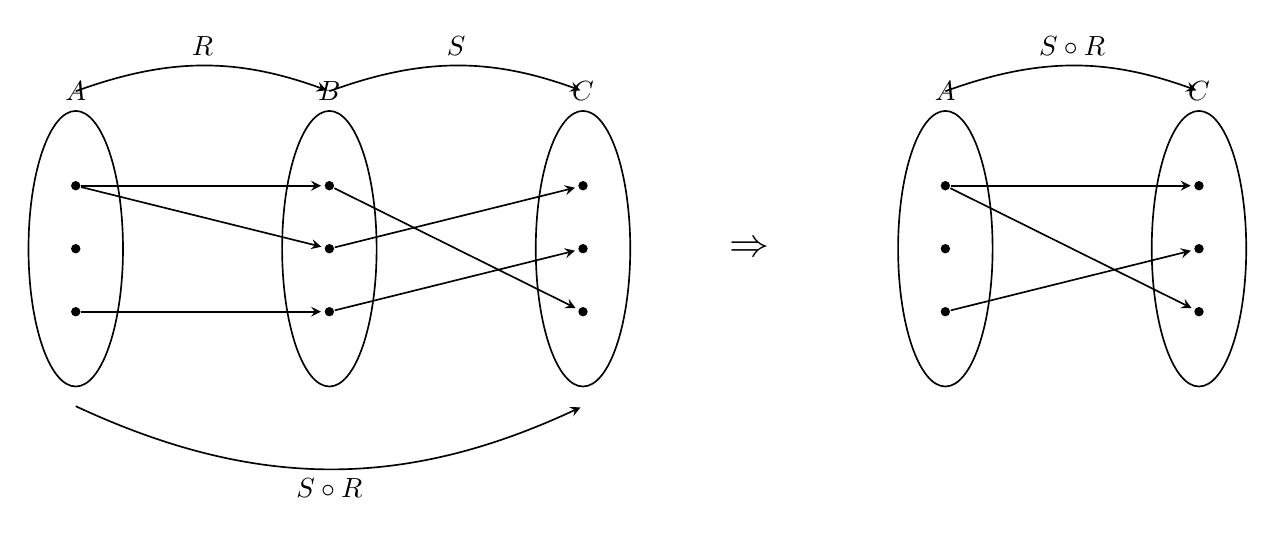
\begin{tikzpicture}[
    > = stealth, % Clean arrowheads
    shorten > = 1pt, % Prevents arrows from touching the dots
    auto,
    node distance = 2cm, 
    semithick,
    set/.style={ellipse, draw, minimum width=1.2cm, minimum height=3.5cm},
    dot/.style={circle, fill, inner sep=1.2pt}
]

% --- LEFT SIDE: A -> B -> C ---
% Draw the sets
\node[set, label=above:$A$] (A) {};
\node[set, right=of A, label=above:$B$] (B) {};
\node[set, right=of B, label=above:$C$] (C) {};

% Draw the elements (dots) in A
\node[dot] (a1) at ([yshift=0.8cm]A.center) {};
\node[dot] (a2) at (A.center) {};
\node[dot] (a3) at ([yshift=-0.8cm]A.center) {};

% Draw the elements (dots) in B
\node[dot] (b1) at ([yshift=0.8cm]B.center) {};
\node[dot] (b2) at (B.center) {};
\node[dot] (b3) at ([yshift=-0.8cm]B.center) {};

% Draw the elements (dots) in C
\node[dot] (c1) at ([yshift=0.8cm]C.center) {};
\node[dot] (c2) at (C.center) {};
\node[dot] (c3) at ([yshift=-0.8cm]C.center) {};

% Draw internal mapping arrows
\draw[->] (a1) -- (b1);
\draw[->] (a1) -- (b2);
\draw[->] (a3) -- (b3);

\draw[->] (b1) -- (c3);
\draw[->] (b2) -- (c1);
\draw[->] (b3) -- (c2);

% Draw top and bottom label arrows
\draw[->, bend left=20] ([yshift=2cm]A.center) to node[above] {$R$} ([yshift=2cm]B.center);
\draw[->, bend left=20] ([yshift=2cm]B.center) to node[above] {$S$} ([yshift=2cm]C.center);
\draw[->, bend right=25] ([yshift=-2cm]A.center) to node[below] {$S \circ R$} ([yshift=-2cm]C.center);

% --- MIDDLE: The Implies Arrow ---
\node (implies) at ([xshift=1.5cm]C.east) {\Large $\Rightarrow$};

% --- RIGHT SIDE: S o R ---
% Draw the sets
\node[set, right=1.5cm of implies, label=above:$A$] (A2) {};
\node[set, right=of A2, label=above:$C$] (C2) {};

% Draw the elements (dots) in A2
\node[dot] (a21) at ([yshift=0.8cm]A2.center) {};
\node[dot] (a22) at (A2.center) {};
\node[dot] (a23) at ([yshift=-0.8cm]A2.center) {};

% Draw the elements (dots) in C2
\node[dot] (c21) at ([yshift=0.8cm]C2.center) {};
\node[dot] (c22) at (C2.center) {};
\node[dot] (c23) at ([yshift=-0.8cm]C2.center) {};

% Draw internal mapping arrows for the composition
\draw[->] (a21) -- (c23); % mapped from a1 -> b1 -> c3
\draw[->] (a21) -- (c21); % mapped from a1 -> b2 -> c1
\draw[->] (a23) -- (c22); % mapped from a3 -> b3 -> c2

% Draw top label arrow
\draw[->, bend left=20] ([yshift=2cm]A2.center) to node[above] {$S \circ R$} ([yshift=2cm]C2.center);

\end{tikzpicture}
\end{center}

\begin{table}[h]
    \centering
    \begin{tabular}{ll}
        \toprule
        \textbf{Proposition} & \textbf{Formula} \\
        \midrule
        Composition is Associative & $T \circ (S \circ R) = (T \circ S) \circ R = T \circ S \circ R$ \\
        Inverse of Composition & $(S \circ R)^{-1} = R^{-1} \circ S^{-1}$ \\
        \bottomrule
    \end{tabular}
    \caption{Properties of Composition (where $R \subseteq A \times B, S \subseteq B \times C, T \subseteq C \times D$)}
\end{table}

\subsection{Properties of Relations}

\begin{definition}[n-ary Relations]
    Given $n$ sets $A_1, A_2, \dots, A_n$, an $n$-ary relation $R$ on $A_1 \times A_2 \times \dots \times A_n$ is a subset of $A_1 \times A_2 \times \dots \times A_n$.
    \begin{itemize}
        \item 2-ary = binary
        \item 3-ary = ternary
        \item 4-ary = quaternary
    \end{itemize}
\end{definition}

\begin{definition}[Reflexivity, Symmetry, and Transitivity]
    Let $R$ be a relation on set $A$.
    \begin{itemize}
        \item $R$ is \textbf{reflexive} iff $\forall x \in A (xRx)$
        \item $R$ is \textbf{symmetric} iff $\forall x, y \in A (xRy \Rightarrow yRx)$
        \item $R$ is \textbf{transitive} iff $\forall x, y, z \in A (xRy \wedge yRz \Rightarrow xRz)$
    \end{itemize}
\end{definition}

\vspace{1em}
\begin{center}
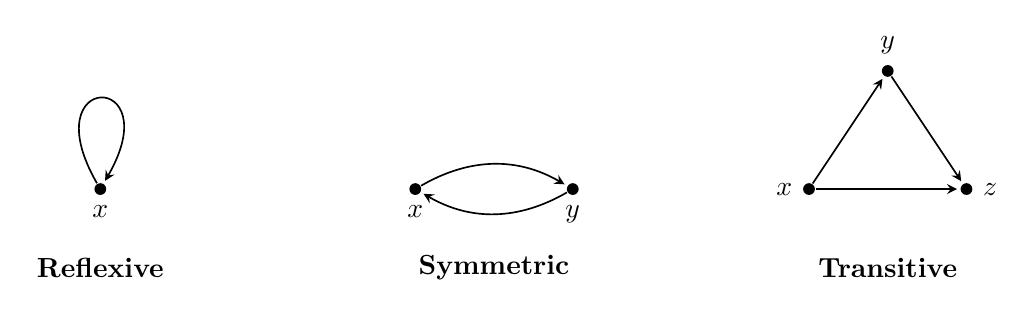
\begin{tikzpicture}[
    > = stealth, 
    shorten > = 1pt, 
    auto, 
    semithick,
    dot/.style={circle, fill, inner sep=1.5pt}
]

% --- Reflexive ---
\begin{scope}[xshift=0cm]
    \node[dot, label=below:$x$] (x1) at (0,0) {};
    % Using looseness and specific out/in angles to make a nice circular loop
    \draw[->] (x1) edge [loop above, out=120, in=60, looseness=50] (x1);
    \node at (0, -1) {\textbf{Reflexive}};
\end{scope}

% --- Symmetric ---
\begin{scope}[xshift=4cm]
    \node[dot, label=below:$x$] (x2) at (0,0) {};
    \node[dot, label=below:$y$] (y2) at (2,0) {};
    \draw[->, bend left=30] (x2) to (y2);
    \draw[->, bend left=30] (y2) to (x2);
    \node at (1, -1) {\textbf{Symmetric}};
\end{scope}

% --- Transitive ---
\begin{scope}[xshift=9cm]
    \node[dot, label=left:$x$] (x3) at (0,0) {};
    \node[dot, label=above:$y$] (y3) at (1, 1.5) {};
    \node[dot, label=right:$z$] (z3) at (2,0) {};
    
    \draw[->] (x3) -- (y3);
    \draw[->] (y3) -- (z3);
    \draw[->] (x3) -- (z3);
    \node at (1, -1) {\textbf{Transitive}};
\end{scope}

\end{tikzpicture}
\end{center}
\vspace{1em}

\begin{definition}[Transitive Closure]
    To obtain a transitive relation, it is necessary to add ordered pairs. The relation obtained by adding the least number of ordered pairs to ensure transitivity is the \textbf{transitive closure} of the relation.
    
    Let $R$ be a relation on set $A$. The transitive closure of $R$, denoted $R^t$ on $A$, satisfies:
    \begin{enumerate}[label=\arabic*.]
        \item $R^t$ is transitive.
        \item $R \subseteq R^t$.
        \item If $S$ is any other transitive relation that contains $R$, then $R^t \subseteq S$.
    \end{enumerate}
\end{definition}

\begin{definition}[More Properties on Relations]
    Let $R$ be a relation on set $A$.
    \begin{itemize}
        \item $R$ is \textbf{asymmetric} iff $\forall x, y \in A (xRy \Rightarrow y \not R x)$
        \item $R$ is \textbf{irreflexive} iff $\forall x \in A (x \not R x)$ ($\neq$ not reflexive)
        \item $R$ is \textbf{antitransitive} iff $\forall x, y, z \in A (xRy \wedge yRz \Rightarrow x \not R z)$
    \end{itemize}
\end{definition}

\subsection{Equivalence Relations and Partitions}

\begin{definition}[Partition]
    A partition of set $A$ is a set of non-empty subsets of $A$ s.t.
    \[ \forall x \in A, \exists! S \in C (x \in S) \]
    ``Every element is in a component $S$ which is an element of partition $C$.''
\end{definition}

\begin{remark}[Bell Numbers]
    The number of partitions of a set with $n$ elements follows the Bell numbers: 1, 1, 2, 5, 15, 52, 203, 877, 4140 \dots
\end{remark}

\begin{definition}[Partitions as Relations]
    A partition can be viewed as an ``is in the same component as'' relation. 
    Given a partition $C$ of a set $A$, the relation $R$ induced by the partition is defined on $A$ as:
    \[ \forall x, y \in A, xRy \Leftrightarrow \exists \text{ component } S \text{ of } C \text{ s.t. } x, y \in S \]
\end{definition}

\begin{theorem}[8.3.1: Relation induced by a partition]
    The relation $R$ on set $A$ induced by the partition is an equivalence relation.
\end{theorem}

\begin{definition}[Equivalence Relations]
    A relation on a set is an equivalence relation iff it is reflexive, symmetric, and transitive. Usually denoted by $\sim$ (e.g., $x \sim y$).
\end{definition}

\begin{definition}[Equivalence Classes]
    Given an equivalence relation $\sim$ on set $A$. For each $a \in A$, the equivalence class of $a$, denoted $[a]_\sim$, is the set of all elements $x \in A$ such that $a \sim x$.
    \[ [a]_\sim = \{x \in A : a \sim x\} \]
    \[ \forall x \in A (x \in [a]_\sim \Leftrightarrow a \sim x) \]
\end{definition}

\begin{lemma}[Rel.1: Equivalence Classes]
    Let $\sim$ be an equivalence relation on set $A$. $\forall x,y \in A$:
    \[ x \sim y \Leftrightarrow [x] = [y] \Leftrightarrow [x] \cap [y] \neq \emptyset \]
\end{lemma}

\begin{theorem}[8.3.4: The partition induced by an equivalence relation]
    Given an equivalence relation $R$ on set $A$, then the distinct equivalence classes of $R$ form a partition of $A$. The union of all equivalence classes of $R$ is $A$, and distinct equivalence classes are mutually disjoint.
\end{theorem}

\begin{example}
    Let Set $A = \{1,2,3,4,5,6\}$ \\
    Partition $C = \{\{1,2,3\}, \{4\}, \{5,6\}\}$ \\
    Components = $\{1,2,3\}$ and $\{4\}$ and $\{5,6\}$
    
    The induced equivalence relation $\sim$ is: 
    \[ \{(1,1), (1,2), (1,3), (2,1), (2,2), (2,3), (3,1), (3,2), (3,3), (4,4), (5,5), (5,6), (6,5), (6,6)\} \]
    
    The equivalence classes are:
    \begin{itemize}
        \item $[1] = [2] = [3] = \{1,2,3\}$ (by Lemma Rel.1)
        \item $[4] = \{4\}$
        \item $[5] = [6] = \{5,6\}$
    \end{itemize}
    
    The set of equivalence classes $A/\sim \ = \{\{1,2,3\}, \{4\}, \{5,6\}\}$.
\end{example}

% Delete and draw by hand
\vspace{1em}
\begin{center}
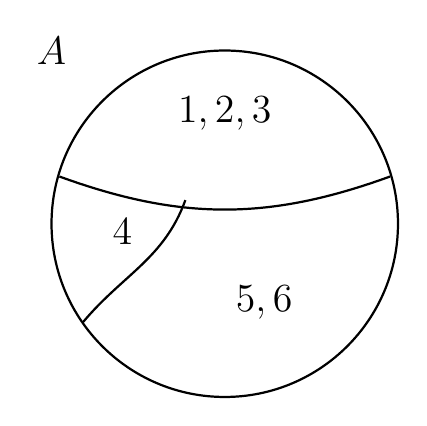
\begin{tikzpicture}[thick]
    % Draw the main set A (the outer circle)
    \draw (0,0) circle (2.2cm);
    
    % Label the set A outside the top left
    \node at (-2.2, 2.2) {\Large $A$};

    % Draw the partition lines using curved paths
    % Top divider
    \draw (-2.1, 0.6) to[out=-20, in=200] (2.1, 0.6);
    % Bottom left divider
    \draw (-1.8, -1.25) to[out=50, in=250] (-0.5, 0.3);

    % Place the elements inside their respective components
    \node at (0, 1.4) {\Large $1, 2, 3$};
    \node at (-1.3, -0.1) {\Large $4$};
    \node at (0.5, -1.0) {\Large $5, 6$};
\end{tikzpicture}
\end{center}
\vspace{1em}

\subsection{Congruence}
Let $a, b \in \mathbb{Z}$ and $n \in \mathbb{Z}^+$. Then $a$ is congruent to $b$ modulo $n$ iff $a - b = nk$ for some $k \in \mathbb{Z}$.
\[ n \mid (a - b) \]
\[ a \equiv b \pmod{n} \]

\begin{proposition}
    Congruence modulo $n$ is an equivalence relation on $\mathbb{Z}$ for every $n \in \mathbb{Z}^+$.
\end{proposition}

\subsubsection{Set of Equivalence Classes}
Let $\sim$ be an equivalence relation on a set $A$. $A/\sim$ is the set of all equivalence classes w.r.t. $\sim$, i.e.,
\[ A/\sim \ = \{[x]_\sim : x \in A\} \]

\begin{theorem}[Rel.2: Equivalence Classes form a Partition]
    Let $\sim$ be an equivalence relation on a set $A$. Then $A/\sim$ is a partition of $A$.
\end{theorem}

\subsection{Partial Order Relations}

\begin{definition}[Antisymmetry]
    Let $R$ be a relation on set $A$. $R$ is \textbf{antisymmetric} iff
    \[ \forall x, y \in A (xRy \wedge yRx \Rightarrow x = y) \]
\end{definition}

\begin{note}
    Antisymmetric $\neq$ Not Symmetric. 
(e.g., Tut 5 Q6(c): $R$ is asymmetric $\Rightarrow R$ is antisymmetric).
\end{note} 

\vspace{1em}
\begin{center}
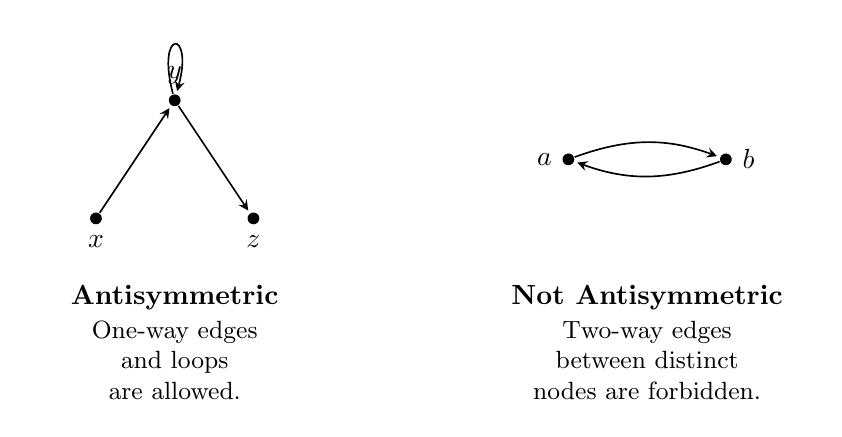
\begin{tikzpicture}[
    > = stealth,
    shorten > = 1pt,
    auto,
    semithick,
    dot/.style={circle, fill, inner sep=1.5pt}
]

% --- Antisymmetric (Valid) ---
\begin{scope}[xshift=0cm]
    \node[dot, label=below:$x$] (x) at (0,0) {};
    \node[dot, label=above:$y$] (y) at (1, 1.5) {};
    \node[dot, label=below:$z$] (z) at (2,0) {};

    % One-way arrows are fine
    \draw[->] (x) -- (y);
    \draw[->] (y) -- (z);
    % Loops are fine
    \draw[->] (y) edge [loop above, looseness=50] (y);

    \node at (1, -1) {\textbf{Antisymmetric}};
    \node[align=center, font=\small, text width=3.5cm] at (1, -1.8) {One-way edges and loops \\ are allowed.};
\end{scope}

% --- Not Antisymmetric (Invalid) ---
\begin{scope}[xshift=6cm]
    \node[dot, label=left:$a$] (a) at (0, 0.75) {};
    \node[dot, label=right:$b$] (b) at (2, 0.75) {};

    % Two-way arrows violate antisymmetry
    \draw[->, bend left=20] (a) to (b);
    \draw[->, bend left=20] (b) to (a);

    \node at (1, -1) {\textbf{Not Antisymmetric}};
    \node[align=center, font=\small, text width=4cm] at (1, -1.8) {Two-way edges between distinct \\ nodes are forbidden.};
\end{scope}

\end{tikzpicture}
\end{center}
\vspace{1em}

\begin{definition}[Partial Order Relation]
    A relation $R$ on set $A$ is a \textbf{partial order relation} iff $R$ is reflexive, antisymmetric, and transitive.
\end{definition}

\begin{note}
    The 2 fundamental partial order relations are $\leq$ and $\subseteq$.
\end{note}

\begin{definition}[Partially Ordered Set (Poset)]
    A set $A$ is a partially ordered set (or poset) w.r.t. a partial order relation $R$ on $A$, denoted by $(A, R)$.
\end{definition}
\textbf{Notation:} $\preceq$ is used to refer to a general partial order. $x \preceq y$ is read ``$x$ is curly less than or equal to $y$''.

\subsection{Hasse Diagrams}
A Hasse diagram is a simplified directed graph for partial order relations.

\textbf{Steps to construct:}
Start with a directed graph of the relation, s.t. all arrows point upward. Then eliminate:
\begin{enumerate}[label=\arabic*.]
    \item The loops at all the vertices (reflexivity is implied).
    \item All arrows whose existence is implied by transitivity (i.e., if arrows for $aRb$ and $bRc$ exist, remove the arrow for $aRc$).
    \item Direction indicators on all arrows (antisymmetry is implied).
\end{enumerate}

\vspace{1em}
\begin{center}
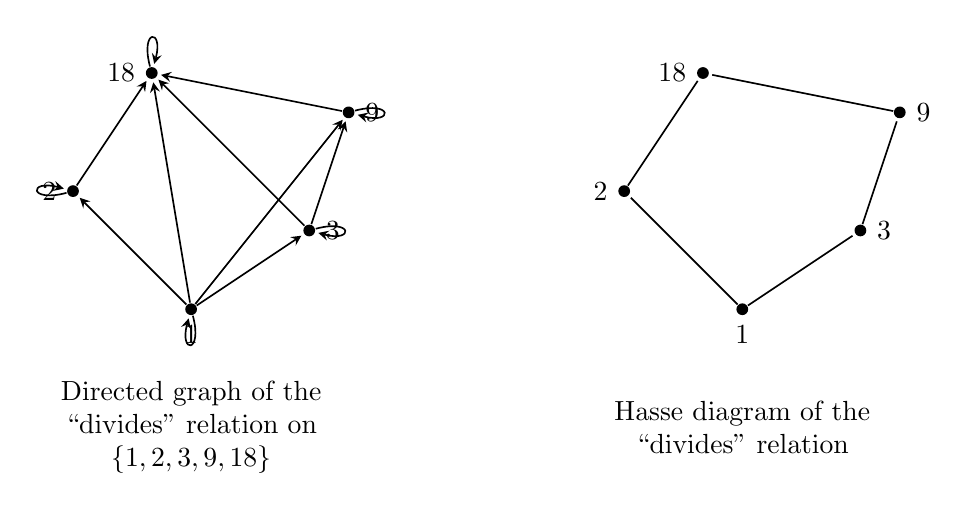
\begin{tikzpicture}[
    > = stealth,
    shorten > = 1pt,
    auto,
    semithick,
    dot/.style={circle, fill, inner sep=1.5pt}
]

% --- Left: Directed Graph ---
\begin{scope}[xshift=0cm]
    \node[dot, label=below:$1$] (1a) at (0,0) {};
    \node[dot, label=left:$2$] (2a) at (-1.5, 1.5) {};
    \node[dot, label=right:$3$] (3a) at (1.5, 1) {};
    \node[dot, label=right:$9$] (9a) at (2, 2.5) {};
    \node[dot, label=left:$18$] (18a) at (-0.5, 3) {};

    % Loops
    \draw[->] (1a) edge [loop below] (1a);
    \draw[->] (2a) edge [loop left] (2a);
    \draw[->] (3a) edge [loop right] (3a);
    \draw[->] (9a) edge [loop right] (9a);
    \draw[->] (18a) edge [loop above] (18a);

    % Edges
    \draw[->] (1a) -- (2a);
    \draw[->] (1a) -- (3a);
    \draw[->] (1a) -- (9a);
    \draw[->] (1a) -- (18a);
    \draw[->] (3a) -- (9a);
    \draw[->] (3a) -- (18a);
    \draw[->] (2a) -- (18a);
    \draw[->] (9a) -- (18a);
    
    \node[align=center, yshift=-1.5cm] at (0,0) {Directed graph of the \\ ``divides'' relation on \\ $\{1,2,3,9,18\}$};
\end{scope}

% --- Right: Hasse Diagram ---
\begin{scope}[xshift=7cm]
    \node[dot, label=below:$1$] (1b) at (0,0) {};
    \node[dot, label=left:$2$] (2b) at (-1.5, 1.5) {};
    \node[dot, label=right:$3$] (3b) at (1.5, 1) {};
    \node[dot, label=right:$9$] (9b) at (2, 2.5) {};
    \node[dot, label=left:$18$] (18b) at (-0.5, 3) {};

    % Edges (no arrows for Hasse)
    \draw (1b) -- (2b);
    \draw (1b) -- (3b);
    \draw (3b) -- (9b);
    \draw (2b) -- (18b);
    \draw (9b) -- (18b);
    
    \node[align=center, yshift=-1.5cm] at (0,0) {Hasse diagram of the \\ ``divides'' relation};
\end{scope}

\end{tikzpicture}
\end{center}
\vspace{1em}

\begin{definition}[Comparability]
    Let $\preceq$ be a partial order on a set $A$. For $a,b \in A$, $a$ and $b$ are \textbf{comparable} iff $a \preceq b$ or $b \preceq a$. Otherwise, $a$ and $b$ are noncomparable.
\end{definition}

\begin{definition}[Maximal / Minimal / Largest / Smallest]
    Let set $A$ be a partially ordered set w.r.t. a relation $\preceq$ and $c \in A$.
    \begin{enumerate}[label=\arabic*.]
        \item $c$ is a \textbf{maximal} element of $A$ iff $\forall x \in A (c \preceq x \Rightarrow c = x)$. (``Nobody can be above $c$, except $c$'').
        \item $c$ is a \textbf{minimal} element of $A$ iff $\forall x \in A (x \preceq c \Rightarrow c = x)$. (``Nobody can be below $c$, except $c$'').
        \item $c$ is the \textbf{largest} element of $A$ iff $\forall x \in A (x \preceq c)$. (``$c$ is above everybody'').
        \item $c$ is the \textbf{smallest} element of $A$ iff $\forall x \in A (c \preceq x)$. (``$c$ is below everybody'').
    \end{enumerate}
\end{definition}
    
\begin{note}
    If $c$ is the smallest element, it is automatically minimal. If $c$ is the largest element, it is automatically maximal.
\end{note}

\subsection{Total Order Relations}
\begin{definition}[Total Order]
    Let $R$ be a partial order relation on set $A$. If for any 2 elements $x, y \in A$, either $xRy$ or $yRx$, then $R$ is a Total Order Relation on $A$.
    
    $R$ is a total order iff $R$ is a partial order and $\forall x, y \in A (xRy \vee yRx)$. (i.e., all elements in $A$ are comparable).
\end{definition}

\begin{definition}[Linearisation of Partial Orders]
    A linearisation of a partial order can be seen as deriving a total order (among many) from that partial order.
    
    Let $\preceq$ be a partial order on a set $A$. A linearisation of $\preceq$ is a total order $\preceq^*$ on $A$ s.t.
    \[ \forall x,y \in A (x \preceq y \Rightarrow x \preceq^* y) \]
\end{definition}

\begin{definition}[Well-Ordered Set]
    Let $\preceq$ be a total order on a set $A$. $A$ is well-ordered iff every non-empty subset contains a smallest element.
    \[ \forall S \in \mathcal{P}(A), S \neq \emptyset \Rightarrow (\exists x \in S, \forall y \in S (x \preceq y)) \]
\end{definition}

\textbf{Examples:}
\begin{itemize}
    \item $(\mathbb{N}, \leq)$ is well-ordered. $\{0, 1, 2, 3, 4, \dots\}$
    \item $(\mathbb{Z}, \leq)$ is \textbf{not} well-ordered. $\{\dots, -1, 0, 1, 2, \dots\}$
\end{itemize}

\section{Functions}

\subsection{Function Basics}

\begin{definition}[Function]
    A function $f$ from set $X$ to set $Y$, denoted $f: X \rightarrow Y$, is a relation that satisfies:
    \begin{enumerate}
        \item[(F1)] $\forall x \in X, \exists y \in Y$ s.t. $(x,y) \in f$
        \item[(F2)] $\forall x \in X, \forall y_1, y_2 \in Y (((x, y_1) \in f \wedge (x, y_2) \in f) \Rightarrow y_1 = y_2)$
    \end{enumerate}
    \textbf{OR}\\
    Let $f$ be a relation on sets $X$ and $Y$ (i.e., $f \subseteq X \times Y$). Then $f$ is a function $f: X \rightarrow Y$ iff
    \[ \forall x \in X, \exists! y \in Y \text{ s.t. } (x,y) \in f \]
    i.e., A function from $X$ to $Y$ is an assignment from each element of $X$ to exactly \textbf{one} element of $Y$.
\end{definition}

\begin{definition}[Image / Preimage]
    Let $f$ be a function from set $X$ to set $Y$ s.t. $f: X \rightarrow Y$. Then $f(x) = y$ iff $(x,y) \in f$.
    \begin{itemize}
        \item $x$ is the \textbf{argument} of $f$.
        \item $f(x)$ is the \textbf{output} of $f$ for the input $x$, or $f(x)$ is the \textbf{image} of $x$ under $f$.
        \item If $f(x) = y$, then $x$ is a \textbf{preimage} of $y$.
    \end{itemize}
\end{definition}

\begin{definition}[Setwise Image / Preimage]
    Given $f: X \rightarrow Y$:
    \begin{itemize}
        \item If $A \subseteq X$, then let $f(A) = \{f(x) : x \in A\} =$ the \textbf{setwise image} of $A$.
        \item If $B \subseteq Y$, then let $f^{-1}(B) = \{x \in X : f(x) \in B\} =$ the \textbf{setwise preimage} of $B$ under $f$.
    \end{itemize}
\end{definition}
\begin{remark}
    $f^{-1}(B)$ does \textbf{not} refer to inverse function. Context will make it clear, but usually a Set means Preimage, an element means inverse function.
\end{remark}

\begin{definition}[Domain, Co-domain, Range]
    Given $f: X \rightarrow Y$:
    \begin{itemize}
        \item $X$ is the \textbf{domain} of $f$ and $Y$ is the \textbf{co-domain} of $f$.
        \item The \textbf{range} of $f$ is the setwise image of $X$ under $f$:
        \[ \{y \in Y : y = f(x) \text{ for some } x \in X\} \]
    \end{itemize}
\end{definition}

\subsection{Sequences and Strings}

\begin{definition}[Sequence]
    A sequence $a_0, a_1, a_2, \dots$ can be represented by a function $a$ whose domain is $\mathbb{Z}_{\geq 0}$ that satisfies $a(n) = a_n$ for every $n \in \mathbb{Z}_{\geq 0}$.
    
    \textbf{Example:} The sequence 2, 3, 5, 9, 17, 33, 65\dots can be represented by the function $a: \mathbb{Z}_{\geq 0} \rightarrow \mathbb{Z}^+$ that satisfies $a(n) = 2^n + 1$.
\end{definition}

\begin{definition}[Equality of Sequences]
    Given 2 sequences represented by the functions $a(n) = a_n$ and $b(n) = b_n$ respectively for every $n \in \mathbb{Z}_{\geq 0}$, the 2 sequences are equal iff $a(n) = b(n)$ for every $n \in \mathbb{Z}_{\geq 0}$.
\end{definition}

\begin{definition}[String]
    Let $A$ be a set. A string over $A$ is an expression of the form $a_0 a_1 a_2 \dots a_{l-1}$ where $l \in \mathbb{Z}_{\geq 0}$ and $a_0, a_1, \dots, a_{l-1} \in A$.
    \begin{itemize}
        \item $l$ represents the length of the string.
        \item $\epsilon$ represents the empty string (length 0).
        \item $A^*$ denotes the set of all strings over $A$.
    \end{itemize}
\end{definition}

\begin{definition}[Equality of Strings]
    Given 2 strings $s_1 = a_0 a_1 \dots a_{l-1}$ and $s_2 = b_0 b_1 \dots b_{l-1}$, $s_1 = s_2$ iff $a_i = b_i$ for all $0 \leq i < l$.
\end{definition}

\begin{theorem}[7.1.1: Function Equality]
    Two functions $f: A \rightarrow B$ and $g: C \rightarrow D$ are equal (i.e., $f=g$) iff:
    \begin{enumerate}
        \item $A = C \wedge B = D$ (Domains and co-domains match)
        \item $f(x) = g(x) \ \forall x \in A$
    \end{enumerate}
\end{theorem}

\subsection{Injections, Surjections, and Bijections}

\begin{definition}[Injections (One-to-One)]
    A function $f: X \rightarrow Y$ is an \textbf{injection} iff:
    \[ \forall x_1, x_2 \in X (f(x_1) = f(x_2) \Rightarrow x_1 = x_2) \]
    or equivalently, via contrapositive:
    \[ x_1 \neq x_2 \Rightarrow f(x_1) \neq f(x_2) \]
    (Each element in the domain has a unique image).
\end{definition}

\begin{definition}[Surjections (Onto)]
    A function $f: X \rightarrow Y$ is \textbf{surjective} iff:
    \[ \forall y \in Y, \exists x \in X (y = f(x)) \]
    (Every element in the co-domain has a preimage. So, Range = Co-domain).
\end{definition}

\begin{definition}[Bijection]
    A function $f: X \rightarrow Y$ is a \textbf{bijection} iff $f$ is both injective and surjective.
    \[ \forall y \in Y, \exists! x \in X (y = f(x)) \]
\end{definition}

% --- FUNCTION DIAGRAMS ---
\vspace{1em}
\begin{center}
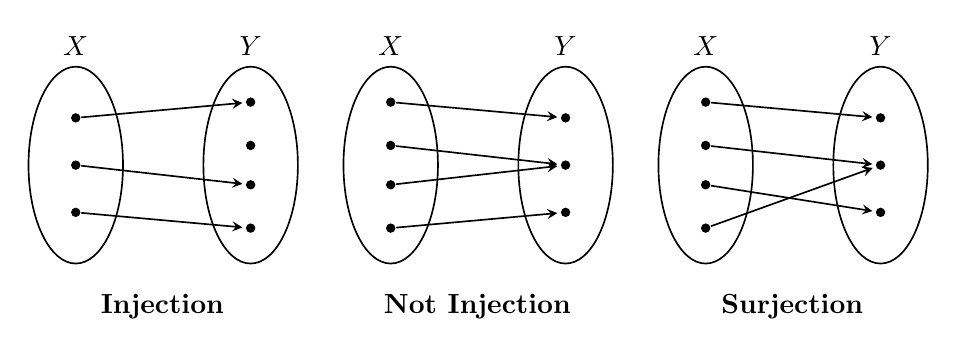
\begin{tikzpicture}[
    > = stealth, shorten > = 1pt, auto, semithick,
    set/.style={ellipse, draw, minimum width=1.2cm, minimum height=2.5cm},
    dot/.style={circle, fill, inner sep=1.2pt}
]

% 1. INJECTION
\begin{scope}[xshift=0cm]
    \node[set, label=above:$X$] (X1) {};
    \node[set, right=1cm of X1, label=above:$Y$] (Y1) {};
    \node at (1.1, -1.8) {\textbf{Injection}};
    
    \node[dot] (x1a) at ([yshift=0.6cm]X1.center) {};
    \node[dot] (x1b) at (X1.center) {};
    \node[dot] (x1c) at ([yshift=-0.6cm]X1.center) {};
    
    \node[dot] (y1a) at ([yshift=0.8cm]Y1.center) {};
    \node[dot] (y1b) at ([yshift=0.25cm]Y1.center) {};
    \node[dot] (y1c) at ([yshift=-0.25cm]Y1.center) {};
    \node[dot] (y1d) at ([yshift=-0.8cm]Y1.center) {};
    
    \draw[->] (x1a) -- (y1a);
    \draw[->] (x1b) -- (y1c);
    \draw[->] (x1c) -- (y1d);
\end{scope}

% 2. NOT INJECTION
\begin{scope}[xshift=4cm]
    \node[set, label=above:$X$] (X2) {};
    \node[set, right=1cm of X2, label=above:$Y$] (Y2) {};
    \node at (1.1, -1.8) {\textbf{Not Injection}};
    
    \node[dot] (x2a) at ([yshift=0.8cm]X2.center) {};
    \node[dot] (x2b) at ([yshift=0.25cm]X2.center) {};
    \node[dot] (x2c) at ([yshift=-0.25cm]X2.center) {};
    \node[dot] (x2d) at ([yshift=-0.8cm]X2.center) {};
    
    \node[dot] (y2a) at ([yshift=0.6cm]Y2.center) {};
    \node[dot] (y2b) at (Y2.center) {};
    \node[dot] (y2c) at ([yshift=-0.6cm]Y2.center) {};
    
    \draw[->] (x2a) -- (y2a);
    \draw[->] (x2b) -- (y2b);
    \draw[->] (x2c) -- (y2b); % Collision!
    \draw[->] (x2d) -- (y2c);
\end{scope}

% 3. SURJECTION
\begin{scope}[xshift=8cm]
    \node[set, label=above:$X$] (X3) {};
    \node[set, right=1cm of X3, label=above:$Y$] (Y3) {};
    \node at (1.1, -1.8) {\textbf{Surjection}};
    
    \node[dot] (x3a) at ([yshift=0.8cm]X3.center) {};
    \node[dot] (x3b) at ([yshift=0.25cm]X3.center) {};
    \node[dot] (x3c) at ([yshift=-0.25cm]X3.center) {};
    \node[dot] (x3d) at ([yshift=-0.8cm]X3.center) {};
    
    \node[dot] (y3a) at ([yshift=0.6cm]Y3.center) {};
    \node[dot] (y3b) at (Y3.center) {};
    \node[dot] (y3c) at ([yshift=-0.6cm]Y3.center) {};
    
    \draw[->] (x3a) -- (y3a);
    \draw[->] (x3b) -- (y3b);
    \draw[->] (x3c) -- (y3c);
    \draw[->] (x3d) -- (y3b);
\end{scope}
\end{tikzpicture}

\vspace{1em}

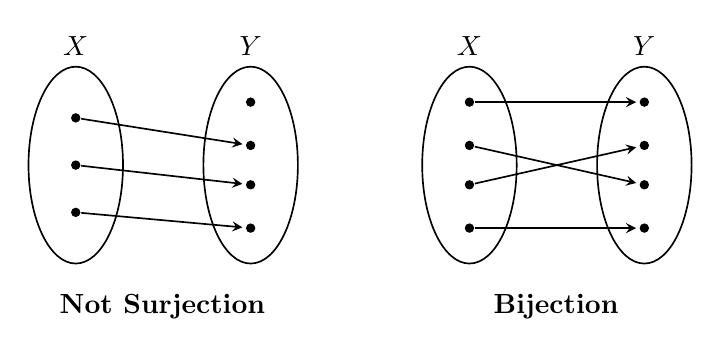
\begin{tikzpicture}[
    > = stealth, shorten > = 1pt, auto, semithick,
    set/.style={ellipse, draw, minimum width=1.2cm, minimum height=2.5cm},
    dot/.style={circle, fill, inner sep=1.2pt}
]
% 4. NOT SURJECTION
\begin{scope}[xshift=0cm]
    \node[set, label=above:$X$] (X4) {};
    \node[set, right=1cm of X4, label=above:$Y$] (Y4) {};
    \node at (1.1, -1.8) {\textbf{Not Surjection}};
    
    \node[dot] (x4a) at ([yshift=0.6cm]X4.center) {};
    \node[dot] (x4b) at (X4.center) {};
    \node[dot] (x4c) at ([yshift=-0.6cm]X4.center) {};
    
    \node[dot] (y4a) at ([yshift=0.8cm]Y4.center) {};
    \node[dot] (y4b) at ([yshift=0.25cm]Y4.center) {};
    \node[dot] (y4c) at ([yshift=-0.25cm]Y4.center) {};
    \node[dot] (y4d) at ([yshift=-0.8cm]Y4.center) {};
    
    \draw[->] (x4a) -- (y4b);
    \draw[->] (x4b) -- (y4c);
    \draw[->] (x4c) -- (y4d);
    % y4a is left empty
\end{scope}

% 5. BIJECTION
\begin{scope}[xshift=5cm]
    \node[set, label=above:$X$] (X5) {};
    \node[set, right=1cm of X5, label=above:$Y$] (Y5) {};
    \node at (1.1, -1.8) {\textbf{Bijection}};
    
    \node[dot] (x5a) at ([yshift=0.8cm]X5.center) {};
    \node[dot] (x5b) at ([yshift=0.25cm]X5.center) {};
    \node[dot] (x5c) at ([yshift=-0.25cm]X5.center) {};
    \node[dot] (x5d) at ([yshift=-0.8cm]X5.center) {};
    
    \node[dot] (y5a) at ([yshift=0.8cm]Y5.center) {};
    \node[dot] (y5b) at ([yshift=0.25cm]Y5.center) {};
    \node[dot] (y5c) at ([yshift=-0.25cm]Y5.center) {};
    \node[dot] (y5d) at ([yshift=-0.8cm]Y5.center) {};
    
    \draw[->] (x5a) -- (y5a);
    \draw[->] (x5b) -- (y5c);
    \draw[->] (x5c) -- (y5b);
    \draw[->] (x5d) -- (y5d);
\end{scope}

\end{tikzpicture}
\end{center}
\vspace{1em}

\subsection{Inverse Functions and Composition}

\begin{definition}[Inverse Functions]
    Let $f: X \rightarrow Y$. Then $f^{-1}: Y \rightarrow X$ is an inverse of $f$ iff:
    \[ \forall x \in X, \forall y \in Y (y = f(x) \Leftrightarrow x = f^{-1}(y)) \]
\end{definition}

\textbf{Uniqueness of Inverses:} If $g_1$ and $g_2$ are inverses of $f: X \rightarrow Y$, then $g_1 = g_2$.

\begin{theorem}[7.2.3: Bijectivity and Invertibility]
    If $f: X \rightarrow Y$ is a bijection, then $f^{-1}: Y \rightarrow X$ is also a bijection.
    i.e., $f: X \rightarrow Y$ is bijective \textbf{iff} $f$ has an inverse.
\end{theorem}

\begin{definition}[Composition of Functions]
    Let $f: X \rightarrow Y$ and $g: Y \rightarrow Z$ be functions. Define a new function $g \circ f: X \rightarrow Z$ as follows:
    \[ (g \circ f)(x) = g(f(x)) \ \forall x \in X \]
\end{definition}

\begin{definition}[Identity Functions]
    The identity function on $X$, $id_X: X \rightarrow X$, is defined as:
    \[ id_X(x) = x \text{ for all } x \in X \]
\end{definition}

\begin{theorem}[7.3.1: Composition with an Identity Function]
    Let $f: X \rightarrow Y$. Suppose $id_X$ and $id_Y$ are identity functions on $X$ and $Y$ respectively, then:
    \[ f \circ id_X = f \quad \text{and} \quad id_Y \circ f = f \]
\end{theorem}

\begin{theorem}[7.3.2: Composition of a function with its inverse]
    If $f: X \rightarrow Y$ is bijective with the inverse $f^{-1}: Y \rightarrow X$, then:
    \[ f^{-1} \circ f = id_X \quad \text{and} \quad f \circ f^{-1} = id_Y \]
\end{theorem}

\begin{definition}[Order of a Function]
    The order of a bijection $f: A \rightarrow A$ is defined to be the smallest $n \in \mathbb{Z}^+$ s.t. 
    \[ \underbrace{f \circ f \circ f \circ \dots \circ f}_{n \text{ times}} = id_A \]
    (Also denoted as $f^n = id_A$).
\end{definition}

\begin{proposition}[Associativity of Function Composition]
    Let $f: A \rightarrow B, g: C \rightarrow D, h: E \rightarrow F$. Then,
    \[ (h \circ g) \circ f = h \circ (g \circ f) \]
\end{proposition}

\begin{proposition}[Non-commutativity of Function Composition]
    Let $f: A \rightarrow B, g: C \rightarrow D$. Then generally,
    \[ f \circ g \neq g \circ f \]
\end{proposition}

\begin{theorem}[7.3.3: Composition of Injections]
    If $f: X \rightarrow Y$ and $g: Y \rightarrow Z$ are both injective, then $g \circ f$ is injective.
\end{theorem}

\begin{theorem}[7.3.4: Composition of Surjections]
    If $f: X \rightarrow Y$ and $g: Y \rightarrow Z$ are both surjective, then $g \circ f$ is surjective.
\end{theorem}

\subsection{Addition and Multiplication on $\mathbb{Z}_n$}
Define addition $+$ and multiplication $\cdot$ on $\mathbb{Z}_n$ as follows:
Whenever $[x], [y] \in \mathbb{Z}_n$,
\[ [x] + [y] = [x + y] \quad \text{and} \quad [x] \cdot [y] = [x \cdot y] \]

\begin{proposition}[Addition on $\mathbb{Z}_n$ is well-defined]
    For all $n \in \mathbb{Z}^+$ and all $[x_1], [y_1], [x_2], [y_2] \in \mathbb{Z}_n$:
    \[ ([x_1] = [x_2] \wedge [y_1] = [y_2]) \Rightarrow ([x_1] + [y_1] = [x_2] + [y_2]) \]
\end{proposition}

\begin{proposition}[Multiplication on $\mathbb{Z}_n$ is well-defined]
    For all $n \in \mathbb{Z}^+$ and all $[x_1], [y_1], [x_2], [y_2] \in \mathbb{Z}_n$:
    \[ ([x_1] = [x_2] \wedge [y_1] = [y_2]) \Rightarrow ([x_1] \cdot [y_1] = [x_2] \cdot [y_2]) \]
\end{proposition}

\newpage

\section{Mathematical Induction}

\subsection{Summation and Product}

\begin{definition}[Summation]
    Given $m, n \in \mathbb{Z}$ and $m \leq n$,
    \[ \sum_{k=m}^{n} a_k = a_m + a_{m+1} + \dots + a_n \]
    $k$ is the index, $m$ is the lower limit, and $n$ is the upper limit of the summation.
    
    Recursive properties:
    \[ \sum_{k=m}^{m} a_k = a_m \quad \text{and} \quad \sum_{k=m}^{n} a_k = \left(\sum_{k=m}^{n-1} a_k\right) + a_n \]
\end{definition}

\begin{definition}[Product]
    Given $m, n \in \mathbb{Z}$ and $m \leq n$,
    \[ \prod_{k=m}^{n} a_k = a_m \cdot a_{m+1} \cdot \dots \cdot a_n \]
    
    Recursive properties:
    \[ \prod_{k=m}^{m} a_k = a_m \quad \text{and} \quad \prod_{k=m}^{n} a_k = \left(\prod_{k=m}^{n-1} a_k\right) \cdot a_n \]
\end{definition}

\begin{theorem}[5.1.1: Properties of Summations and Products]
    Given $m, n \in \mathbb{Z}$, $m \leq n$, and $c \in \mathbb{R}$:
    \begin{enumerate}[label=\arabic*.]
        \item $\displaystyle \sum_{k=m}^{n} a_k + \sum_{k=m}^{n} b_k = \sum_{k=m}^{n} (a_k + b_k)$
        \item $\displaystyle c \cdot \sum_{k=m}^{n} a_k = \sum_{k=m}^{n} c \cdot a_k$
        \item $\displaystyle \left(\prod_{k=m}^{n} a_k\right) \cdot \left(\prod_{k=m}^{n} b_k\right) = \prod_{k=m}^{n} (a_k \cdot b_k)$
    \end{enumerate}
\end{theorem}

\textbf{Change of Variable Example:}
\[ \sum_{k=1}^{3} k^2 = \sum_{k=3}^{5} (k-2)^2 \]

\subsection{Sequences}

\begin{definition}[Arithmetic Sequence]
    A sequence $a_0, a_1, a_2, \dots$ is called an arithmetic sequence iff there is a constant $d$ such that:
    \[ a_k = a_{k-1} + d \quad \text{for all integers } k \geq 1 \]
    and
    \[ a_n = a_0 + dn \quad \text{for all integers } n \geq 0 \]
    $d$ is the \textbf{common difference} and $a_0$ is the \textbf{initial term}.
\end{definition}

\begin{definition}[Geometric Sequence]
    A sequence $a_0, a_1, a_2, \dots$ is called a geometric sequence iff there is a constant $r$ such that:
    \[ a_k = r \cdot a_{k-1} \quad \text{for all integers } k \geq 1 \]
    and
    \[ a_n = a_0 r^n \quad \text{for all integers } n \geq 0 \]
    $r$ is the \textbf{common ratio} and $a_0$ is the \textbf{initial term}.
\end{definition}

\subsection{Mathematical Induction}

\begin{definition}[Principle of Mathematical Induction]
    Let $P(n)$ be a property that is defined for integers $n$, and let $a$ be a fixed integer.
    Suppose the following are true:
    \begin{enumerate}[label=\arabic*.]
        \item $P(a)$ is true.
        \item For all integers $k \geq a$, if $P(k)$ is true, then $P(k+1)$ is true.
    \end{enumerate}
    Then the statement ``for all integers $n \geq a, P(n)$'' is true.
\end{definition}

\textbf{Method of Proof by Mathematical Induction}
\begin{itemize}
    \item \textbf{Step 1 (Basis Step):} Show that $P(a)$ is true.
    \item \textbf{Step 2 (Inductive Step):} Show that for all integers $k \geq a$, if $P(k)$ is true then $P(k+1)$ is true.
    \begin{itemize}
        \item First, suppose that $P(k)$ is true, where $k$ is any particular but arbitrarily chosen integer with $k \geq a$ [\textbf{Inductive Hypothesis}].
        \item Then show that $P(k+1)$ is true.
    \end{itemize}
    \item \textbf{Step 3:} Conclude that $P(n)$ is true for all $n \geq a$.
\end{itemize}

\begin{theorem}[5.2.2: Sum of first $n$ integers]
    For all integers $n \geq 1$,
    \[ 1 + 2 + 3 + \dots + n = \frac{n(n+1)}{2} \]
\end{theorem}

\begin{definition}[Principle of Strong Mathematical Induction]
    Let $P(n)$ be a property that is defined for integers $n$, and let $a$ and $b$ be fixed integers with $a \leq b$. Suppose the following are true:
    \begin{enumerate}[label=\arabic*.]
        \item $P(a), P(a+1), \dots, P(b)$ are true (\textbf{Basis Step}).
        \item For any integer $k \geq b$, if $P(i)$ is true for all integers $i$ from $a$ through $k$, then $P(k+1)$ is true (\textbf{Inductive Step}).
    \end{enumerate}
    Then the statement ``for all integers $n \geq a, P(n)$'' is true.
\end{definition}

\subsubsection{Weak (1PI) VS Strong (2PI) Induction}

\begin{table}[h]
    \centering
    \begin{tabular}{p{0.3\textwidth} p{0.35\textwidth} p{0.3\textwidth}}
        \toprule
        \textbf{1PI (Weak)} & \textbf{2PI (Strong)} & \textbf{2PI Variant} \\
        \midrule
        \textbf{If} & \textbf{If} & \textbf{If} \\
        $P(a)$ holds & $P(a)$ holds & $P(a), P(a+1), \dots, P(b)$ hold \\
        \addlinespace
        For every $k \geq a$, \newline $P(k) \Rightarrow P(k+1)$ & For every $k \geq a$, \newline $(P(a) \wedge P(a+1) \wedge \dots \wedge P(k)) \Rightarrow P(k+1)$ & For every $k \geq a$, \newline $P(k) \Rightarrow P(k+b-a+1)$ \\
        \addlinespace
        \textbf{Then} & \textbf{Then} & \textbf{Then} \\
        $P(n)$ holds for every $n \geq a$. & $P(n)$ holds for every $n \geq a$. & $P(n)$ holds for every $n \geq a$. \\
        \bottomrule
    \end{tabular}
    \caption{Comparison of Induction Principles}
    \label{tab:induction_types}
\end{table}

\subsection{Recurrence Relations and Recursion}

\begin{definition}[Recurrence Relation]
    A recurrence relation for a sequence $a_0, a_1, a_2, \dots$ is a formula that relates each term $a_k$ to certain of its predecessors $a_{k-i}$, where $i$ is an integer with $k-i \geq 0$.
\end{definition}

\begin{definition}[Recursively Defined Sets]
    Recursive Definition of a set $S$:
    \begin{enumerate}
        \item \textbf{(Base Clause)} Specify that certain elements, called \textit{founders}, are in $S$. If $c$ is a founder, then $c \in S$.
        \item \textbf{(Recursion Clause)} Specify certain functions, called \textit{constructors}, under which the set $S$ is closed. If $f$ is a constructor and $x \in S$, then $f(x) \in S$.
        \item \textbf{(Minimality Clause)} Membership for $S$ can always be demonstrated by (infinitely many) successive applications of the clauses above.
    \end{enumerate}
\end{definition}

\begin{definition}[Structural Induction over $S$]
    To prove that $\forall x \in S, P(x)$ is true, where each $P(x)$ is a proposition, it suffices to:
    \begin{enumerate}
        \item \textbf{(Basis Step)} Show that $P(c)$ is true for every founder $c$.
        \item \textbf{(Induction Step)} Show that $\forall x \in S (P(x) \Rightarrow P(f(x)))$ is true for every constructor $f$.
    \end{enumerate}
    If all founders satisfy a property $P$, and $P$ is preserved by all constructors, then all elements of $S$ satisfy $P$.
\end{definition}

\section{Cardinality}

\subsection{The Pigeonhole Principle}

\begin{theorem}[Pigeonhole Principle]
    Let $A$ and $B$ be finite sets. If there is an injection $f: A \rightarrow B$, then $|A| \leq |B|$. \\
    \textit{Informal:} ``If there are $m$ pigeons put into $n$ pigeonholes and $m > n$, then there must be (at least) one pigeonhole with (at least) 2 pigeons.''
\end{theorem}

\begin{theorem}[Dual Pigeonhole Principle]
    Let $A$ and $B$ be finite sets. If there is a surjection $f: A \rightarrow B$, then $|A| \geq |B|$. \\
    \textit{Informal:} ``If there are $m$ pigeons put into $n$ pigeonholes and $m < n$, then there must be (at least) one pigeonhole with no pigeons.''
\end{theorem}

\subsection{Finite Sets \& Cardinality}

\begin{definition}[Finite Sets]
    Let $\mathbb{Z}_n = \{1, 2, 3, \dots, n\}$, the set of all positive integers from 1 to $n$. \\
    A set $S$ is said to be \textbf{finite} iff $S$ is empty, or there exists a bijection from $S$ to $\mathbb{Z}_n$ for some $n \in \mathbb{Z}^+$.
\end{definition}
*Note: Two finite sets whose elements can be paired by a bijection have the same size.

\begin{definition}[Cardinality]
    The Cardinality of a finite set $S$, denoted $|S|$, is:
    \begin{enumerate}[label=(\roman*)]
        \item 0 if $S = \emptyset$
        \item $n$ if there is a bijection $f: S \rightarrow \mathbb{Z}_n$
    \end{enumerate}
\end{definition}

\begin{theorem}[Equality of Cardinality of Finite Sets]
    Let $A$ and $B$ be any finite sets.
    \[ |A| = |B| \text{ \textbf{iff} there is a bijection } f: A \rightarrow B \]
    *Note: This can be generalized to infinite sets by Cantor's definition of Same Cardinality.
\end{theorem}

\begin{theorem}[7.4.1: Properties of Cardinality]
    The Cardinality relation is an equivalence relation. For all sets $A, B, C$:
    \begin{enumerate}[label=\alph*.]
        \item \textbf{Reflexive:} $|A| = |A|$
        \item \textbf{Symmetric:} $|A| = |B| \Rightarrow |B| = |A|$
        \item \textbf{Transitive:} $(|A| = |B|) \wedge (|B| = |C|) \Rightarrow (|A| = |C|)$
    \end{enumerate}
\end{theorem}

\begin{note}
    An infinite set can have the same cardinality as a proper subset of itself.
\end{note}

\subsection{Countable and Uncountable Sets}

\begin{definition}[Countably Infinite]
    The set $A$ having the same cardinality as $\mathbb{Z}^+$ is called \textbf{countably infinite}. \\
    $A$ has the same cardinality as $\mathbb{Z}^+$ because there is a bijection $f: \mathbb{Z}^+ \rightarrow A$.
    \begin{itemize}
        \item Because $f$ is injective, every element of $A$ is counted at most once.
        \item Because $f$ is surjective, every element of $A$ is counted at least once.
    \end{itemize}
\end{definition}

\vspace{1em}
\begin{center}
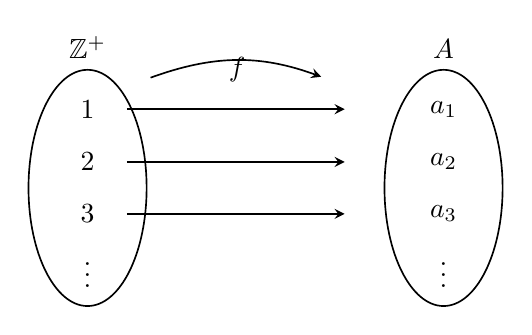
\begin{tikzpicture}[
    > = stealth, shorten > = 1pt, auto, semithick,
    set/.style={ellipse, draw, minimum width=1.5cm, minimum height=3cm},
    dot/.style={circle, fill, inner sep=1.2pt}
]
    \node[set, label=above:$\mathbb{Z}^+$] (Z) {};
    \node[set, right=3cm of Z, label=above:$A$] (A) {};
    
    \node at (Z.center) [yshift=1cm] {$1$};
    \node at (Z.center) [yshift=0.33cm] {$2$};
    \node at (Z.center) [yshift=-0.33cm] {$3$};
    \node at (Z.center) [yshift=-1cm] {$\vdots$};
    
    \node at (A.center) [yshift=1cm] {$a_1$};
    \node at (A.center) [yshift=0.33cm] {$a_2$};
    \node at (A.center) [yshift=-0.33cm] {$a_3$};
    \node at (A.center) [yshift=-1cm] {$\vdots$};

    \draw[->] (0.5, 1) -- (3.3, 1);
    \draw[->] (0.5, 0.33) -- (3.3, 0.33);
    \draw[->] (0.5, -0.33) -- (3.3, -0.33);
    
    \node at (1.9, 1.5) {$f$};
    \draw[->, bend left=20] (0.8, 1.4) to (3.0, 1.4);
\end{tikzpicture}
\end{center}
\vspace{1em}

\begin{definition}[Cardinal Numbers]
    Define $\aleph_0 = |\mathbb{Z}^+|$ (``aleph-nought''). It is the first cardinal number. \\
    A set $S$ is said to be countably infinite iff $|S| = \aleph_0$.
\end{definition}

\begin{definition}[Countable Set]
    A set is said to be \textbf{countable} iff it is finite OR countably infinite. \\
    A set is \textbf{uncountable} if it is not countable.
\end{definition}

\subsubsection{Important Countable Sets}

\textbf{1. $\mathbb{Z}$ is countable} \\
The bijection $f: \mathbb{Z}^+ \rightarrow \mathbb{Z}$ can be defined as:
\[
f(n) = 
\begin{cases} 
    n/2 & \text{if } n \text{ is an even positive integer} \\
    -(n-1)/2 & \text{if } n \text{ is an odd positive integer}
\end{cases}
\]

\textbf{2. $\mathbb{Q}^+$ is countable} \\
Define a function $f: \mathbb{Z}^+ \rightarrow \mathbb{Q}^+$ by starting to count at $1/1$ in a grid layout and following a diagonal snake path, skipping over any number (fraction equivalent) that has already been counted.
\begin{itemize}
    \item \textbf{Injectivity:} Every positive rational number appears somewhere in the grid and will be counted eventually.
    \item \textbf{Surjectivity:} Skipping numbers that have already been counted ensures no number is counted twice.
\end{itemize}
Hence $\mathbb{Z}^+ \rightarrow \mathbb{Q}^+$ is a bijection. So $\mathbb{Q}^+$ is countably infinite.

\vspace{1em}
\begin{center}
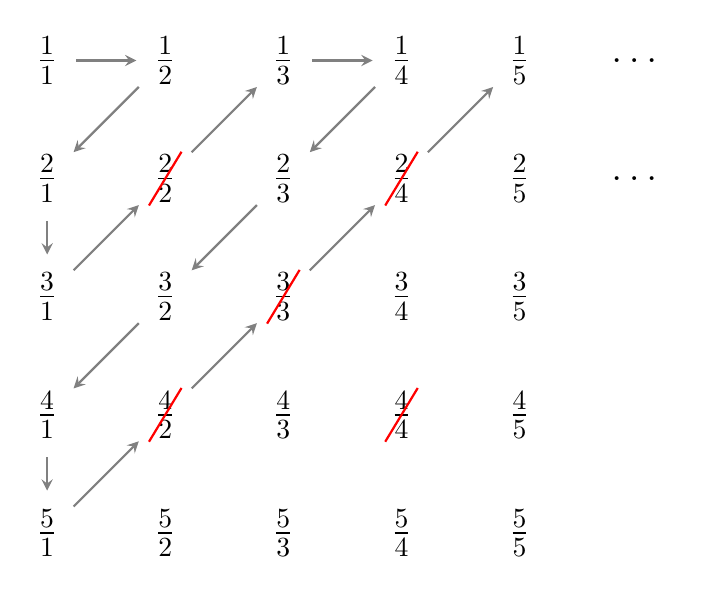
\begin{tikzpicture}[
    > = stealth,
    shorten > = 3pt,
    shorten < = 3pt,
    auto,
    thick
]

% 1. Create the grid of fractions using nested loops
\foreach \row in {1, 2, 3, 4, 5} {
    \foreach \col in {1, 2, 3, 4, 5} {
        % Position each node at (x, -y) to match standard reading order
        \node (\row-\col) at (\col*1.5, -\row*1.5) {\Large $\frac{\row}{\col}$};
    }
}

% 2. Add the continuation dots on the right
\node at (6*1.5, -1*1.5) {\Large $\dots$};
\node at (6*1.5, -2*1.5) {\Large $\dots$};

% 3. Cross out the non-simplified fractions (duplicates)
\draw[red, thick] (2-2.south west) -- (2-2.north east);
\draw[red, thick] (2-4.south west) -- (2-4.north east);
\draw[red, thick] (3-3.south west) -- (3-3.north east);
\draw[red, thick] (4-2.south west) -- (4-2.north east);
\draw[red, thick] (4-4.south west) -- (4-4.north east);

% 4. Draw the zigzag path arrows
\draw[->, gray] (1-1) -- (1-2);

\draw[->, gray] (1-2) -- (2-1);

\draw[->, gray] (2-1) -- (3-1);

\draw[->, gray] (3-1) -- (2-2);
\draw[->, gray] (2-2) -- (1-3);

\draw[->, gray] (1-3) -- (1-4);

\draw[->, gray] (1-4) -- (2-3);
\draw[->, gray] (2-3) -- (3-2);
\draw[->, gray] (3-2) -- (4-1);

\draw[->, gray] (4-1) -- (5-1);

\draw[->, gray] (5-1) -- (4-2);
\draw[->, gray] (4-2) -- (3-3);
\draw[->, gray] (3-3) -- (2-4);
\draw[->, gray] (2-4) -- (1-5);

\end{tikzpicture}
\end{center}
\vspace{1em}

\textbf{3. $\mathbb{Z}^+ \times \mathbb{Z}^+$ is countable} \\
The bijection $f: \mathbb{Z}^+ \times \mathbb{Z}^+ \rightarrow \mathbb{Z}^+$ can be defined as:
\[ f(x,y) = \frac{(x+y-2)(x+y-1)}{2} + x \]

\subsection{Theorems on Countability}

\begin{theorem}[Cartesian Product]
    If sets $A$ and $B$ are both countably infinite, then so is $A \times B$.
\end{theorem}

\begin{corollary}[General Cartesian Product]
    Given $n \geq 2$ countably infinite sets $A_1, A_2, \dots, A_n$, the Cartesian Product $A_1 \times A_2 \times \dots \times A_n$ is also countably infinite.
\end{corollary}

\begin{theorem}[Unions]
    The union of countably many countable sets is also countable. \\
    If $A_1, A_2, A_3, \dots$ are all countable sets, then so is $\bigcup_{i - 1}^{\infty} A_i$.
\end{theorem}

\subsection{Summary of Previous Proofs}
\begin{itemize}
    \item If $B$ is countably infinite and $C$ is finite, $B \cup C$ is countable. \textit{(Tutorial \#8 Q2)}
    \item Let $S_i$ be a countably infinite set for each $i \in \mathbb{Z}^+$. Then $\bigcup_{i \in \mathbb{Z}^+} S_i$ is countable. \textit{(Tutorial \#8 Q5)}
    \item A set $B$ is infinite iff there is a proper subset $A \subset B$ s.t. $|A| = |B|$. \textit{(Tutorial \#8 Q7)}
    \item $\mathbb{C}$ (the set of complex numbers) is uncountable. \textit{(Tutorial \#8 Q8)}
    \item If $A$ is countably infinite, $\mathcal{P}(A)$ is uncountable. \textit{(Tutorial \#8 Q2)}
    \item If $A$ is countably infinite and $B$ is finite, $A \setminus B$ is countably infinite. \textit{(Assignment \#2 Q4(a))}
    \item Let $A, B, C$ be sets s.t. $A \subseteq B \subseteq C$. If $A$ and $C$ are countably infinite, $B$ is countably infinite. \textit{(Assignment \#2 Q4(c))}
\end{itemize}

\subsection{Countability via Sequences}

\begin{proposition}[9.1]
    An infinite set $B$ is countable iff there is a sequence $b_0, b_1, b_2, \dots \in B$ in which every element of $B$ appears exactly once.
\end{proposition}

\begin{lemma}[9.2: Countability via Sequence]
    An infinite set $B$ is countable iff there is a sequence $b_0, b_1, b_2, \dots$ in which every element of $B$ appears.
\end{lemma}

\subsection{Larger Infinities}

\begin{theorem}[7.4.2: Cantor]
    The set of real numbers between $0$ and $1$,
    \[ (0,1) = \{x \in \mathbb{R} \mid 0 < x < 1\} \]
    is uncountable.
\end{theorem}

\subsubsection*{Cantor's Diagonalization Argument}
\begin{enumerate}
    \item Suppose $(0,1)$ is countable.
    \item Since $(0,1)$ is not finite, it is countably infinite.
    \item List the elements $x_i$ of $(0,1)$ in a sequence as follows:
    \[
        \begin{aligned}
            x_1 &= 0.a_{11}a_{12}a_{13}\dots a_{1n}\dots \\
            x_2 &= 0.a_{21}a_{22}a_{23}\dots a_{2n}\dots \\
            x_3 &= 0.a_{31}a_{32}a_{33}\dots a_{3n}\dots \\
            &\vdots \\
            x_n &= 0.a_{n1}a_{n2}\dots a_{nn}\dots
        \end{aligned}
    \]
    where each $a_{ij} \in \{0, 1, \dots, 9\}$ is a digit.
    \item Now, construct a number $d = 0.d_1 d_2 \dots d_n \dots$ s.t.
    \[
        d_n =
        \begin{cases}
            1, & \text{if } a_{nn} \neq 1 \\
            2, & \text{if } a_{nn} = 1
        \end{cases}
    \]
    \item Note that $\forall n \in \mathbb{Z}^+, d_n \neq a_{nn}$. Thus, $d \neq x_n, \forall n \in \mathbb{Z}^+$.
    \item However $d \in (0,1)$, which is a contradiction. Therefore $(0,1)$ is uncountable.
\end{enumerate}

The list will always be incomplete because there will always be a way to express $d$ as a different real number in the list.

\subsection{Cardinality and Countability}

\begin{theorem}[7.4.3]
    Any subset of any countable set is countable.
\end{theorem}

\begin{corollary}[7.4.4: Contrapositive of Theorem 7.4.3]
    Any set with an uncountable subset is uncountable.
\end{corollary}

\begin{proposition}[9.3]
    Every infinite set has a countably infinite subset.
\end{proposition}

\begin{lemma}[9.4: Union of Countably Infinite Sets]
    Let $A$ and $B$ be countably infinite sets. Then $A \cup B$ is countable.
\end{lemma}

\subsubsection*{Cardinality of $\mathbb{R}$}
\[ |\mathbb{R}| = |(0,1)| \]

\section{Counting I}

A \emph{sample space} is the set of all possible outcomes of a random process or experiment. An \emph{event} is a subset of a sample space.

\begin{theorem}[9.2.1: The Multiplication / Product Rule]
    If an operation consists of $k$ steps and
    \begin{itemize}
        \item the $1^{\text{st}}$ step can be performed in $n_1$ ways,
        \item the $2^{\text{nd}}$ step can be performed in $n_2$ ways,
        \item $\vdots$
        \item the $k^{\text{th}}$ step can be performed in $n_k$ ways,
    \end{itemize}
    Then the entire operation can be performed in $n_1 \times n_2 \times n_3 \times \dots \times n_k$ ways.
\end{theorem}

\begin{theorem}[5.2.4: Sets]
    Suppose $A$ is a finite set. Then $|P(A)| = 2^{|A|}$.
\end{theorem}

\subsubsection*{Principle of Sum (or the Addition Principle)}
If we have $m$ ways of doing something and $n$ ways of doing another thing but both cannot be done at the same time, then there are $m+n$ ways to choose one of these actions.

\begin{theorem}[9.2.2: Permutations]
    The number of permutations of a set with $n$ ($n \geq 1$) elements is $n!$.
\end{theorem}

\subsubsection*{$r$-permutations}
An \emph{$r$-permutation} of a set of $n$ elements is an ordered selection of $r$ elements taken from the set. The number of $r$-permutations of a set of $n$ elements is denoted $P(n,r)$.

\begin{theorem}[9.2.3: $r$-permutations from a set of $n$ elements]
    If $n$ and $r$ are integers and $1 \leq r \leq n$, then the number of $r$-permutations of a set of $n$ elements is given by the formula
    \[ P(n,r) = \frac{n!}{(n-r)!} \]
\end{theorem}

\begin{theorem}[9.3.1: The Addition / Sum Rule]
    Suppose a finite set $A$ equals the union of $k$ distinct mutually disjoint subsets $A_1, A_2, \dots, A_k$. Then $|A| = |A_1| + |A_2| + \dots + |A_k|$.
\end{theorem}

\begin{theorem}[9.2.3: $r$-permutations from a set of $n$ elements]
    If $n$ and $r$ are integers and $1 \leq r \leq n$, then the number of $r$-permutations of a set of $n$ elements is given by the formula
    \[ P(n,r) = \frac{n!}{(n-r)!} \]
\end{theorem}
 
\begin{theorem}[9.3.1: The Addition / Sum Rule]
    Suppose a finite set $A$ equals the union of $k$ distinct mutually disjoint subsets $A_1, A_2, \dots, A_k$. Then $|A| = |A_1| + |A_2| + \dots + |A_k|$.
\end{theorem}
 
\begin{theorem}[9.3.2: The Difference Rule]
    If $A$ is a finite set and $B \subseteq A$, then $|A \setminus B| = |A| - |B|$.
\end{theorem}
 
\begin{theorem}[9.3.3: The Inclusion / Exclusion Rule for 2 or 3 sets]
    If $A$, $B$, and $C$ are finite sets, then
    \[ |A \cup B| = |A| + |B| - |A \cap B| \]
    and
    \[ |A \cup B \cup C| = |A| + |B| + |C| - |A \cap B| - |A \cap C| - |B \cap C| + |A \cap B \cap C| \]
\end{theorem}
 
\subsubsection*{Generalized Pigeonhole Principle}
For any function $f$ from a finite set $X$ with $n$ elements to a finite set $Y$ with $m$ elements and for any positive integer $k$, if $k < n/m$, then there is some $y \in Y$ s.t. $y$ is the image of at least $k+1$ distinct elements of $X$.
 
\subsubsection*{Generalized Pigeonhole Principle (Contrapositive)}
For any function $f$ from a finite set $X$ with $n$ elements to a finite set $Y$ with $m$ elements and for any positive integer $k$, if for each $y \in Y$, $f^{-1}(\{y\})$ has at most $k$ elements, then $X$ has at most $km$ elements. $n \leq km$.
 
\subsubsection*{Summation from 1 to $n$}
\[ \sum_{i=1}^{n} i = \frac{n(n+1)}{2} \]
 
\section{Counting II}
 
\subsection{$r$-combinations}
Let $n$ and $r$ be non-negative integers with $r \leq n$. An \emph{$r$-combination} of a set of $n$ elements is a subset of $r$ of the $n$ elements. $\binom{n}{r}$ denotes the number of subsets of size $r$ ($r$-combinations) that can be chosen from a set of $n$ elements.
 
\begin{theorem}[9.5.1: Formula for $\binom{n}{r}$]
    \[ \binom{n}{r} = \frac{P(n,r)}{r!} \]
    \[ \binom{n}{r} = \frac{n!}{r!(n-r)!} \]
\end{theorem}
 
\begin{theorem}[9.5.2: Permutations with sets of indistinguishable objects]
    Suppose a collection consists of $n$ objects of which
    \begin{itemize}
        \item $n_1$ are of type 1 and are indistinguishable from each other
        \item $n_2$ are of type 2 and are \dots
        \item $\vdots$
        \item $n_k$ are of type $k$ and are \dots
    \end{itemize}
    and suppose that $n_1 + n_2 + \dots + n_k = n$. Then the number of distinguishable permutations of the $n$ objects is
    \[ \binom{n}{n_1}\binom{n-n_1}{n_2}\binom{n-n_1-n_2}{n_3} \dots \binom{n-n_1-\dots-n_{k-1}}{n_k} = \frac{n!}{n_1! n_2! \dots n_k!} \]
\end{theorem}
 
\subsubsection*{$r$-combinations with repetition}
 
\paragraph{Multiset}
An \emph{$r$-combination with repetition allowed}, or multiset of size $r$, chosen from a set $X$ of $n$ elements is an unordered selection of elements taken from $X$ with repetition allowed. If $X = \{x_1, x_2, \dots, x_n\}$, we write an $r$-combination with repetition allowed as $[x_{i_1}, x_{i_2}, \dots, x_{i_r}]$ where each $x_{i_j}$ is in $X$ and some of the $x_{i_j}$ may equal each other.
 
\begin{theorem}[9.6.1: Number of $r$-combinations with repetition allowed]
    The number of $r$-combinations with repetition allowed (multisets of size $r$) that can be selected from a set of $n$ elements is:
    \[ \binom{r+n-1}{r} \]
    $\equiv$ the number of ways $r$ objects can be selected from $n$ categories of objects with repetition allowed.
\end{theorem}
 
\subsubsection*{Formulae}
\begin{center}
\begin{tabular}{|c|c|c|}
    \hline
    & Order Matters & Order does not Matter \\
    \hline
    Repetition Allowed & $n^k$ & $\binom{k+n-1}{k}$ \\
    \hline
    Repetition not Allowed & $P(n,k)$ & $\binom{n}{k}$ \\
    \hline
\end{tabular}
\end{center}
 
\begin{theorem}[9.7.1: Pascal's Formula]
    Let $n$ and $r$ be positive integers, $r \leq n$. Then,
    \[ \binom{n+1}{r} = \binom{n}{r-1} + \binom{n}{r} \]
\end{theorem}
 
\begin{theorem}[9.7.2: Binomial Theorem]
    Given $a, b \in \mathbb{R}$ and $n \in \mathbb{Z}_{\geq 0}$
    \[ (a+b)^n = \sum_{k=0}^{n} \binom{n}{k} a^{n-k} b^k \]
    \[ = a^n + \binom{n}{1}a^{n-1}b^1 + \binom{n}{2}a^{n-2}b^2 + \dots + \binom{n}{n-1}a^1 b^{n-1} + b^n \]
\end{theorem}
 
\subsubsection*{Circular Permutation}
The number of ways to permute $n$ objects in a circle is $(n-1)!$ ways.

\begin{center}
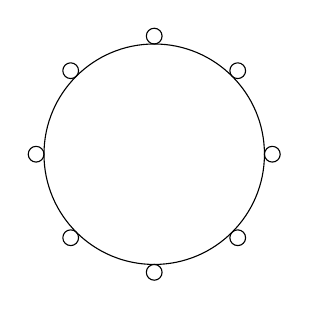
\begin{tikzpicture}
    \foreach \i in {0,...,7} {
        \draw (\i*45:1.5) circle (0.1);
    }
    \draw (0,0) circle (1.4);
\end{tikzpicture}
\end{center}

\section{Probability}
 
\subsection{Probability Axioms}
Let $S$ be a sample space. A probability function $P$ from the set of all events in $S$ to the set of real numbers satisfies the following axioms:
 
For all events $A$ and $B$ in $S$,
\begin{enumerate}
    \item $0 \leq P(A) \leq 1$
    \item $P(\emptyset) = 0$ and $P(S) = 1$
    \item If $A$ and $B$ are disjoint $(A \cap B = \emptyset)$, then $P(A \cup B) = P(A) + P(B)$.
\end{enumerate}
 
\subsubsection*{Probability of the Complement of an Event}
If $A$ is any event in a sample space $S$, then
\[ P(\bar{A}) = 1 - P(A) \]
 
\subsubsection*{Probability of a General Union of Two Events}
If $A$ and $B$ are any events in a sample space $S$, then
\[ P(A \cup B) = P(A) + P(B) - P(A \cap B) \]
 
\subsubsection*{Expected Value}
Suppose the possible outcomes of an experiment, or random process, are real numbers $a_1, a_2, \dots, a_n$ which occur with probabilities $p_1, p_2, \dots, p_n$. The expected value of the process is:
\[ \sum_{k=1}^{n} a_k p_k = a_1 p_1 + a_2 p_2 + \dots + a_n p_n \]
 
\subsubsection*{Linearity of Expectation}
The expected value of the sum of random variables is equal to the sum of their individual expected values, regardless of whether they are independent.
 
For random variables $X$ and $Y$,
\[ E[X+Y] = E[X] + E[Y] \]
 
For random variables $X_1, X_2, \dots, X_n$ and constants $c_1, c_2, \dots, c_n$,
\[ E\left[\sum_{i=1}^{n} c_i \cdot X_i\right] = \sum_{i=1}^{n} (c_i \cdot E[X_i]) \]
 
\subsection{Conditional Probability}
Let $A$ and $B$ be events in a sample space $S$. If $P(A) \neq 0$, then the conditional probability of $B$ given $A$, denoted $P(B|A)$, is
\[ P(B|A) = \frac{P(A \cap B)}{P(A)} \tag{9.9.1} \]
\[ P(A \cap B) = P(B|A) \cdot P(A) \tag{9.9.2} \]
\[ P(A) = \frac{P(A \cap B)}{P(B|A)} \tag{9.9.3} \]
 
\begin{theorem}[9.9.1: Bayes' Theorem]
    Suppose that a sample space $S$ is a union of mutually disjoint events $B_1, B_2, \dots, B_n$. Suppose $A$ is an event in $S$, and $P(A)$ and $P(B_i) \neq 0$. If $k$ is an integer with $1 \leq k \leq n$, then
    \[ P(B_k|A) = \frac{P(A|B_k) \cdot P(B_k)}{P(A|B_1) \cdot P(B_1) + P(A|B_2) \cdot P(B_2) + \dots + P(A|B_n) \cdot P(B_n)} \]
\end{theorem}
 
or,
\[ P(A|B) = \frac{P(B|A) \cdot P(A)}{P(B)} \]
 
\subsubsection*{Independent Events}
If $A$ and $B$ are events in a sample space $S$, then $A$ and $B$ are independent iff
\[ P(A \cap B) = P(A) \cdot P(B) \]
 
\subsubsection*{Pairwise Independent and Mutually Independent}
Let $A, B, C$ be events in a sample space $S$. $A, B$, and $C$ are pairwise independent iff they satisfy conditions 1-3. $A, B$, and $C$ are mutually independent iff they satisfy all four conditions.
\begin{enumerate}
    \item $P(A \cap B) = P(A) \cdot P(B)$
    \item $P(A \cap C) = P(A) \cdot P(C)$
    \item $P(B \cap C) = P(B) \cdot P(C)$
    \item $P(A \cap B \cap C) = P(A) \cdot P(B) \cdot P(C)$
\end{enumerate}
 
\section{Graphs}
 
An undirected graph $G = (V, E)$ consists of
\begin{itemize}
    \item A set of vertices $V = \{v_1, v_2, v_3, \dots, v_n\}$
    \item A set of (undirected) edges $E = \{e_1, e_2, e_3, \dots, e_n\}$
    \item An (undirected) edge $e$ connecting $v_i$ and $v_j$ is denoted as $e = \{v_i, v_j\}$
\end{itemize}
 
\subsubsection*{Undirected Graph}
\begin{itemize}
    \item Each edge is associated with either one or two vertices called its endpoints.
    \item An edge is said to connect its endpoints; two vertices connected by an edge are called adjacent vertices; and a vertex that is an endpoint of a loop is adjacent to itself.
    \item An edge is said to be incident on each of its endpoints, and two edges incident on the same endpoint are adjacent edges.
\end{itemize}
$e = \{v, w\}$ is an undirected edge incident on vertices $v$ and $w$.
 
\subsubsection*{Directed Graph}
A directed graph, or digraph $G$, consists of 2 finite sets. A non-empty set $V$ of vertices and a set $E$ of directed edges, where each directed edge is associated with an ordered pair of vertices called its endpoints.
 
$e = (v, w)$ is a directed edge from vertex $v$ to vertex $w$.
 
\subsubsection*{Simple Graph}
A simple graph is an undirected graph that does not have any loops or parallel edges. (There is at most one edge between each pair of distinct vertices.)
 
\begin{center}
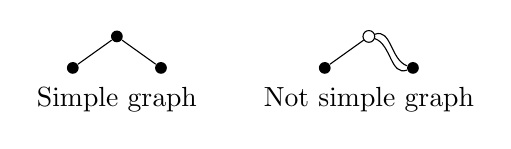
\begin{tikzpicture}[scale=0.8]
   
    \node[circle, fill, inner sep=1.5pt] (a) at (0,0) {};
    \node[circle, fill, inner sep=1.5pt] (b) at (0.7,0.5) {};
    \node[circle, fill, inner sep=1.5pt] (c) at (1.4,0) {};
    \draw (a) -- (b) -- (c);
    \node at (0.7,-0.5) {Simple graph};
 
   
    \node[circle, fill, inner sep=1.5pt] (d) at (4,0) {};
    \node[circle, draw, inner sep=1.5pt, minimum size=4pt] (e) at (4.7,0.5) {};
    \node[circle, fill, inner sep=1.5pt] (f) at (5.4,0) {};
    \draw (d) -- (e);
    \draw (e) to[out=20,in=160] (f);
    \draw (e) to[out=-20,in=200] (f);
    \node at (4.7,-0.5) {Not simple graph};
\end{tikzpicture}
\end{center}
 
\subsubsection*{Complete Graph}
A complete graph on $n$ vertices, $n>0$, denoted $K_n$ is a simple graph with $n$ vertices and exactly one edge connecting each pair of distinct vertices.
 
\begin{center}
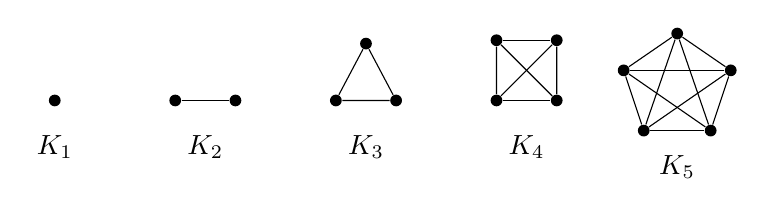
\begin{tikzpicture}[scale=0.85, every node/.style={circle, fill, inner sep=1.5pt}]
   
    \node (k1) at (0,0) {};
    \node at (0,-0.7) [fill=none] {$K_1$};
 
   
    \node (k2a) at (1.8,0) {};
    \node (k2b) at (2.7,0) {};
    \draw (k2a) -- (k2b);
    \node at (2.25,-0.7) [fill=none] {$K_2$};
 
   
    \node (k3a) at (4.2,0) {};
    \node (k3b) at (5.1,0) {};
    \node (k3c) at (4.65,0.85) {};
    \draw (k3a) -- (k3b) -- (k3c) -- (k3a);
    \node at (4.65,-0.7) [fill=none] {$K_3$};
 
   
    \node (k4a) at (6.6,0) {};
    \node (k4b) at (7.5,0) {};
    \node (k4c) at (7.5,0.9) {};
    \node (k4d) at (6.6,0.9) {};
    \draw (k4a) -- (k4b);
    \draw (k4b) -- (k4c);
    \draw (k4c) -- (k4d);
    \draw (k4d) -- (k4a);
    \draw (k4a) -- (k4c);
    \draw (k4b) -- (k4d);
    \node at (7.05,-0.7) [fill=none] {$K_4$};
 
   
    \node (k5a) at (9.3,1.0) {};
    \node (k5b) at (10.1,0.45) {};
    \node (k5c) at (9.8,-0.45) {};
    \node (k5d) at (8.8,-0.45) {};
    \node (k5e) at (8.5,0.45) {};
    \draw (k5a) -- (k5b);
    \draw (k5b) -- (k5c);
    \draw (k5c) -- (k5d);
    \draw (k5d) -- (k5e);
    \draw (k5e) -- (k5a);
    \draw (k5a) -- (k5c);
    \draw (k5a) -- (k5d);
    \draw (k5b) -- (k5d);
    \draw (k5b) -- (k5e);
    \draw (k5c) -- (k5e);
    \node at (9.3,-1.0) [fill=none] {$K_5$};
\end{tikzpicture}
\end{center}
 
\[ \text{no. of edges of } K_n = \frac{n(n-1)}{2} \]
 
\subsubsection*{Subgraph}
A graph $H$ is a subgraph of graph $G$ iff every vertex in $H$ is also a vertex in $G$, every edge in $H$ is also an edge in $G$, and every edge in $H$ has the same endpoints as it has in $G$.
 
\subsubsection*{Degree of a Vertex}
Let $G$ be an undirected graph and $v$ is a vertex in $G$. The degree of $v$, $\deg(v)$, is the number of edges incident on $v$, and an edge that is a loop is counted twice. The total degree of $G$ is the sum of the degrees of all the vertices in $G$.
 
\begin{theorem}[10.1.1: The Handshake Theorem]
    If the vertices of $G$ are $v_1, v_2, \dots, v_n$, where $n \geq 0$, then the total degree of $G = 2 \times$ the number of edges in $G$.
\end{theorem}
 
\begin{corollary}[10.1.2]
    The total degree of a graph is even.
\end{corollary}
 
\begin{proposition}[10.1.3]
    In any graph there are an even number of vertices of odd degree.
\end{proposition}
 
\subsubsection*{Indegree and Outdegree w.r.t. a Directed Graph}
Let $G = (V,E)$ be a directed graph and $v$ be a vertex of $G$. The indegree of $v$, $\deg^-(v)$, is the no. of edges that end at $v$. The outdegree of $v$, $\deg^+(v)$, is the no. of edges that originate from $v$.
\[ \sum_{v \in V} \deg^-(v) = \sum_{v \in V} \deg^+(v) = |E| \]
 
\subsubsection*{Bipartite Graph}
A bipartite graph (or bigraph) is a simple graph whose vertices can be divided into two disjoint sets $U$ and $V$ s.t. every edge connects a vertex $v \in V$ to $w \in W$.
 
\begin{center}
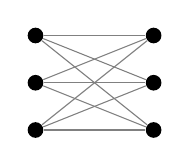
\begin{tikzpicture}[scale=0.6, every node/.style={circle, fill, inner sep=2pt}]
    \foreach \i in {1,2,3} {
        \node (l\i) at (0,-\i) {};
    }
    \foreach \i in {1,2,3} {
        \node (r\i) at (2.5,-\i) {};
    }
    \foreach \i in {1,2,3} {
        \foreach \j in {1,2,3} {
            \draw[gray] (l\i) -- (r\j);
        }
    }
\end{tikzpicture}
\end{center}
 
\subsubsection*{Complete Bipartite Graph}
A complete bipartite graph is a bipartite graph on two disjoint sets $U$ and $V$ s.t. every vertex in $U$ connects to every vertex in $V$. If $|U|=m$ and $|V|=n$, the complete bigraph is denoted $K_{m,n}$. Max. no. of edges of $K_{n,n} = \left\lfloor \dfrac{N^2}{4} \right\rfloor$, $N = n+n$.
 
\begin{center}
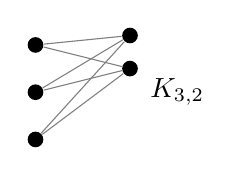
\begin{tikzpicture}[scale=0.6, every node/.style={circle, fill, inner sep=2pt}]
    \foreach \i in {1,2,3} {
        \node (l\i) at (0,-\i) {};
    }
    \foreach \i in {1,2} {
        \node (r\i) at (2,-1.5-\i*0.7+1.4) {};
    }
    \foreach \i in {1,2,3} {
        \foreach \j in {1,2} {
            \draw[gray] (l\i) -- (r\j);
        }
    }
    \node at (3, -2) [fill=none] {$K_{3,2}$};
\end{tikzpicture}
\end{center}
 
\subsection{Trails, Paths, Circuits}
Let $G$ be a graph, and let $v$ and $w$ be vertices of $G$.
 
\subsubsection*{Walk}
A walk from $v$ to $w$ is a sequence of adjacent vertices and edges of $G$, and has the form $v_0, e_0, v_1, e_1, \dots, v_{n-1}, e_n, v_n$. $n$ is the length of the walk.
 
\subsubsection*{Trivial Walk}
A trivial walk from $v$ to $v$ consists of the single vertex $v$.
 
\subsubsection*{Trail}
A trail from $v$ to $w$ is a walk from $v$ to $w$ that does not contain a repeated edge.
 
\subsubsection*{Path}
A path from $v$ to $w$ is a trail that does not contain a repeated vertex.
 
\subsubsection*{Closed Walk}
A closed walk is a walk that starts and ends at the same vertex.
 
\subsubsection*{Circuit / Cycle}
A circuit/cycle is a closed walk of at least length 3 and does not contain a repeated edge.
 
\subsubsection*{Simple Circuit}
A simple circuit/cycle is a circuit that does not have any other repeated vertex except the first and last.
 
An undirected graph is cyclic if it contains a loop or a cycle. Otherwise it is acyclic.
 
\subsubsection*{Connectedness}
Two vertices $v$ and $w$ of a graph $G=(V,E)$ are connected iff there is a walk from $v$ to $w$. The graph $G$ is connected iff given any two vertices $v$ and $w$, there is a walk from $v$ to $w$.
 
\begin{lemma}[10.2.1]
    Let $G$ be a graph.
    \begin{enumerate}
        \item[a.] If $G$ is connected, then any two distinct vertices of $G$ can be connected by a path.
        \item[b.] If vertices $v$ and $w$ are part of a circuit in $G$ and one edge is removed from the circuit, then there still exists a trail from $v$ to $w$ in $G$.
        \item[c.] If $G$ is connected and $G$ contains a circuit, then an edge of the circuit can be removed without disconnecting $G$.
    \end{enumerate}
\end{lemma}
 
\subsubsection*{Connected Component}
($\to$ a connected subgraph of largest possible size)
 
A graph $H$ is a connected component of graph $G$ iff
\begin{enumerate}
    \item $H$ is a subgraph of $G$.
    \item $H$ is connected.
    \item No connected subgraph of $G$ has $H$ as a subgraph and contains vertices or edges not in $H$.
\end{enumerate}
 
\subsection{Euler Circuit / Eulerian Graph}
Let $G$ be a graph. An Euler circuit for $G$ is a circuit that contains every vertex and every edge of $G$.
 
An Eulerian graph is a graph containing an Euler circuit.
 
\begin{theorem}[10.2.2]
    If a graph has an Euler circuit, then every vertex of the graph has positive even degree.
\end{theorem}
 
\paragraph{Contrapositive of 10.2.2:} If some vertex of a graph has odd degree, the graph does not have an Euler circuit.
 
\begin{theorem}[10.2.3]
    If a graph $G$ is connected and the degree of every vertex in $G$ is a positive even integer, $G$ has an Euler circuit.
\end{theorem}
 
\subsubsection*{Euler Trail}
Let $G$ be a graph, $v$ and $w$ be two distinct vertices of $G$. An Euler trail/path from $v$ to $w$ is a sequence of adjacent edges and vertices that starts at $v$, ends at $w$, passes through every vertex of $G$ at least once, and traverses every edge of $G$ exactly once.
 
\begin{corollary}[10.2.5]
    Let $G$ be a graph, and let $v$ and $w$ be two distinct vertices of $G$. There is an Euler trail from $v$ to $w$ iff $G$ is connected, $v$ and $w$ have odd degree, and all other vertices of $G$ have positive even degree.
\end{corollary}
 
\subsection{Hamiltonian Circuit / Hamiltonian Graph}
Given a graph $G$, a Hamiltonian circuit for $G$ is a simple circuit that includes every vertex of $G$ (every vertex appears exactly once, except the first and last which are the same).
 
A Hamiltonian graph is a graph that contains a Hamiltonian Circuit.
 
\begin{proposition}[10.2.6]
    If a graph $G$ has a Hamiltonian circuit, then $G$ has a subgraph $H$ with the following:
    \begin{enumerate}
        \item $H$ contains every vertex of $G$.
        \item $H$ is connected.
        \item $H$ has the same number of edges as vertices.
        \item Every vertex of $H$ has degree 2.
    \end{enumerate}
\end{proposition}
 
\subsubsection*{Catalan's Numbers}
\[ C_n = \frac{1}{n+1}\binom{2n}{n} \]
\begin{enumerate}
    \item No. of full binary trees with $n$ leaves $\to$ $n-1$ internal nodes.
    \item No. of non-isomorphic ordered trees with $n$ vertices.
\end{enumerate}
 
\subsection{Matrices}
 
\subsubsection*{Matrix}
A $m \times n$ (read "m by n") matrix $A$ over a set $S$ is a rectangular array of elements of $S$ arranged into $m$ rows and $n$ columns. We write $\mathbf{A} = (a_{ij})$.
 
\[
\mathbf{A} =
\begin{bmatrix}
a_{11} & a_{12} & \dots & a_{1j} & \dots & a_{1n} \\
a_{21} & a_{22} & \dots & a_{2j} & \dots & a_{2n} \\
\vdots & \vdots & & \vdots & & \vdots \\
a_{i1} & a_{i2} & \dots & a_{ij} & \dots & a_{in} \\
\vdots & \vdots & & \vdots & & \vdots \\
a_{m1} & a_{m2} & \dots & a_{mj} & \dots & a_{mn}
\end{bmatrix}
\]
 
If $\mathbf{A}$ and $\mathbf{B}$ are matrices, then $\mathbf{A} = \mathbf{B}$ if, and only if, $\mathbf{A}$ and $\mathbf{B}$ have the same size and the corresponding entries of $\mathbf{A}$ and $\mathbf{B}$ are all equal; that is, $a_{ij} = b_{ij}$ for all $i = 1,2,\dots,m$ and $j = 1,2,\dots,n$.
 
A matrix for which the numbers of rows and columns are equal is called a \textbf{square matrix}.
 
If $\mathbf{A}$ is a square matrix of size $n \times n$, then the main diagonal of $\mathbf{A}$ consists of all the entries $a_{11}, a_{22}, \dots, a_{nn}$.
 
\subsubsection*{Scalar / Dot Product}
Suppose that all entries in matrices $\mathbf{A}$ and $\mathbf{B}$ are real numbers. If the number of elements, $n$, in the $i$th row of $\mathbf{A}$ equals the number of elements in the $j$th column of $\mathbf{B}$, then the \textbf{scalar product} or \textbf{dot product} of the $i$th row of $\mathbf{A}$ and the $j$th column of $\mathbf{B}$ is the real number obtained as follows:
\[
\begin{bmatrix} a_{i1} & a_{i2} & \dots & a_{in} \end{bmatrix}
\begin{bmatrix} b_{1j} \\ b_{2j} \\ \vdots \\ b_{nj} \end{bmatrix}
= a_{i1}b_{1j} + a_{i2}b_{2j} + \dots + a_{in}b_{nj}
\]
 
\subsubsection*{Matrix Multiplication}
Let $\mathbf{A} = (a_{ij})$ be an $m \times k$ matrix and $\mathbf{B} = (b_{ij})$ a $k \times n$ matrix with real entries. The (matrix) product of $\mathbf{A}$ times $\mathbf{B}$, denoted $\mathbf{AB}$, is that matrix $(c_{ij})$ defined as follows:
 
\[
\scalebox{0.76}{$
\begin{bmatrix}
a_{11} & a_{12} & \dots & a_{1k} \\
a_{21} & a_{22} & \dots & a_{2k} \\
\vdots & \vdots & & \vdots \\
\fbox{$a_{i1}$} & \fbox{$a_{i2}$} & \fbox{$\dots$} & \fbox{$a_{ik}$} \\
\vdots & \vdots & & \vdots \\
a_{m1} & a_{m2} & \dots & a_{mk}
\end{bmatrix}
\begin{bmatrix}
b_{11} & b_{12} & \dots & \fbox{$b_{1j}$} & \dots & b_{1n} \\
b_{21} & b_{22} & \dots & \fbox{$b_{2j}$} & \dots & b_{2n} \\
\vdots & \vdots & & \fbox{$\vdots$} & & \vdots \\
b_{k1} & b_{k2} & \dots & \fbox{$b_{kj}$} & \dots & b_{kn}
\end{bmatrix}
=
\begin{bmatrix}
c_{11} & c_{12} & \dots & c_{1j} & \dots & c_{1n} \\
c_{21} & c_{22} & \dots & c_{2j} & \dots & c_{2n} \\
\vdots & \vdots & & \vdots & & \vdots \\
c_{i1} & c_{i2} & \dots & \fbox{$c_{ij}$} & \dots & c_{in} \\
\vdots & \vdots & & \vdots & & \vdots \\
c_{m1} & c_{m2} & \dots & c_{mj} & \dots & c_{mn}
\end{bmatrix}
$}
\]
 
where $c_{ij} = a_{i1}b_{1j} + a_{i2}b_{2j} + \dots + a_{ik}b_{kj} = \sum_{r=1}^{k} a_{ir}b_{rj}$ for all $i = 1,2,\dots,m$ and $j = 1,2,\dots,n$.
 
Note: matrix multiplication is \textbf{not commutative} i.e. $\mathbf{A} \times \mathbf{B} \neq \mathbf{B} \times \mathbf{A}$ but it is associative, i.e. $(\mathbf{AB})\mathbf{C} = \mathbf{A}(\mathbf{BC})$.
 
\subsubsection*{Identity Matrix}
For each positive integer $n$, the $n \times n$ identity matrix, denoted $I_n = (\delta_{ij})$ or just $\mathbf{I}$ (if the size of the matrix is obvious from context), is the $n \times n$ matrix in which all the entries in the main diagonal are 1's and all other entries are 0's. In other words,
\[
\delta_{ij} =
\begin{cases}
1, & \text{if } i = j \\
0, & \text{if } i \neq j
\end{cases}
\]
 
\subsubsection*{$n$th Power of a Matrix}
For any $n \times n$ matrix $\mathbf{A}$, the powers of $\mathbf{A}$ are defined as follows: $\mathbf{A}^0 = \mathbf{I}$ where $\mathbf{I}$ is the $n \times n$ identity matrix. $\mathbf{A}^n = \mathbf{A}\mathbf{A}^{n-1}$ for all integers $n \geq 1$.
 
\subsubsection*{Adjacency Matrix of a Directed Graph}
Let $G$ be a directed graph with ordered vertices $v_1, v_2, \dots, v_n$. The \textbf{adjacency matrix} of $G$ is the $n \times n$ matrix $\mathbf{A} = (a_{ij})$ over the set of non-negative integers such that $a_{ij}$ = the number of arrows connecting $v_i$ and $v_j$ for all $i,j = 1,2,\dots,n$.
 
\begin{center}
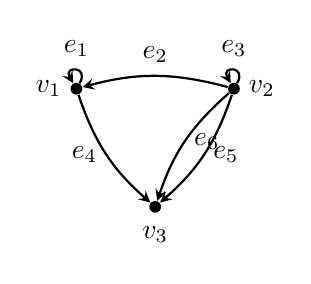
\begin{tikzpicture}[scale=1, >=stealth, every node/.style={circle, fill, inner sep=1.5pt}]
    \node[label=left:$v_1$] (v1) at (0,0) {};
    \node[label=right:$v_2$] (v2) at (2,0) {};
    \node[label=below:$v_3$] (v3) at (1,-1.5) {};
 
   
    \draw[->, thick, black] (v1) to[out=60,in=120,looseness=8] node[fill=none, above] {$e_1$} (v1);
   
    \draw[->, thick, black] (v2) to[out=60,in=120,looseness=8] node[fill=none, above] {$e_3$} (v2);
   
    \draw[->, thick, black] (v2) to[bend right=15] node[fill=none, above] {$e_2$} (v1);
   
    \draw[->, thick, black] (v1) to[bend right=15] node[fill=none, left] {$e_4$} (v3);
   
    \draw[->, thick, black] (v2) to[bend left=15] node[fill=none, right] {$e_5$} (v3);
    \draw[->, thick, black] (v2) to[bend right=15] node[fill=none, right] {$e_6$} (v3);
\end{tikzpicture}
\hspace{1cm}
$\mathbf{A} =
\begin{array}{c}
\begin{array}{ccc} \quad v_1 & v_2 & v_3 \end{array} \\
\begin{array}{c} v_1 \\ v_2 \\ v_3 \end{array}
\begin{bmatrix}
1 & 0 & 0 \\
1 & 1 & 2 \\
1 & 0 & 0
\end{bmatrix}
\end{array}$
 
\vspace{0.3cm}
Directed Graph $G$ \hspace{2.5cm} Adjacency Matrix
\end{center}
 
\subsubsection*{Adjacency Matrix of an Undirected Graph}
Let $G$ be an undirected graph with ordered vertices $v_1, v_2, \dots, v_n$. The adjacency matrix of $G$ is the $n \times n$ matrix $\mathbf{A} = (a_{ij})$ over the set of non-negative integers such that $a_{ij}$ = the number of edges connecting $v_i$ and $v_j$ for all $i,j = 1,2,\dots,n$.
 
Note: the adjacency matrix for an undirected graph is symmetric.
 
\subsubsection*{Symmetric Matrix}
An $n \times n$ square matrix $A = (a_{ij})$ is called \textbf{symmetric} iff for all $i,j = 1,2,\dots,n$, $a_{ij} = a_{ji}$.


 
\subsubsection*{Isomorphic Graph}
Let $G = (V_G, E_G)$ and $G' = (V_{G'}, E_{G'})$ be two graphs. $G$ is \textbf{isomorphic} to $G'$, denoted $G \cong G'$, if and only if there exist bijections $g: V_G \to V_{G'}$ and $h: E_G \to E_{G'}$ that preserve the edge-endpoint functions of $G$ and $G'$ in the sense that for all $v \in V_G$ and $e \in E_G$, $v$ is an endpoint of $e \Leftrightarrow g(v)$ is an endpoint of $h(e)$.
 
\paragraph{Alternative definition of Isomorphic Graph} Let $G = (V_G, E_G)$ and $G' = (V_{G'}, E_{G'})$ be two graphs. $G$ is isomorphic to $G'$ if and only if there exists a permutation $\pi: V_G \to V_{G'}$ such that $\{u,v\} \in E_G \Leftrightarrow \{\pi(u), \pi(v)\} \in E_{G'}$.
 
\subsubsection*{Planar Graph}
A planar graph is a graph that can be drawn on a (two-dimensional) plane without edges crossing.
 
\begin{center}
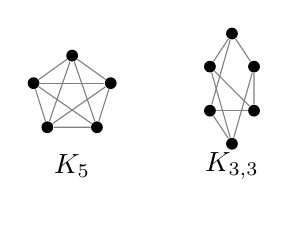
\begin{tikzpicture}[scale=0.7, every node/.style={circle, fill, inner sep=1.5pt}]
   
    \node (k5a) at (8,0.9) [label=above:{}] {};
    \node (k5b) at (8.7,0.4) {};
    \node (k5c) at (8.45,-0.4) {};
    \node (k5d) at (7.55,-0.4) {};
    \node (k5e) at (7.3,0.4) {};
    \draw[gray] (k5a) -- (k5b) -- (k5c) -- (k5d) -- (k5e) -- (k5a);
    \draw[gray] (k5a) -- (k5c);
    \draw[gray] (k5a) -- (k5d);
    \draw[gray] (k5b) -- (k5d);
    \draw[gray] (k5b) -- (k5e);
    \draw[gray] (k5c) -- (k5e);
    \node[fill=none] at (8,-1.1) {$K_5$};
 
   
    \node (l1) at (10.5,0.7) {};
    \node (l2) at (11.3,0.7) {};
    \node (l3) at (10.5,-0.1) {};
    \node (l4) at (11.3,-0.1) {};
    \node (l5) at (10.9,-0.7) {};
    \node (l6) at (10.9,1.3) {};
    \foreach \a in {l1,l2,l3} {
        \foreach \b in {l4,l5,l6} {
            \draw[gray] (\a) -- (\b);
        }
    }
    \node[fill=none] at (10.9,-1.1) {$K_{3,3}$};
\end{tikzpicture}
\end{center}
 
\textbf{Kuratowski's Theorem} A finite graph is planar if and only if it does not contain a subgraph that is a subdivision of the complete graph $K_5$ or the complete bipartite graph $K_{3,3}$.
 
\subsubsection*{Dominating Set}
A set of vertices, $D$, in an undirected simple graph is said to be a \textbf{dominating set} if every vertex not in $D$ is adjacent to at least one vertex in $D$.
 
\subsubsection*{Minimal Dominating Set}
A minimal dominating set is a dominating set such that none of its proper subsets are dominating sets.
 
\subsubsection*{Complement of a Graph}
If $G$ is a simple graph, the \emph{complement} of $G$, denoted $\overline{G}$, is obtained as follows: the vertex set of $\overline{G}$ is identical to the vertex set of $G$. However, two distinct vertices $v$ and $w$ are connected by an edge if and only if $v$ and $w$ are not connected by an edge in $G$.
 
\subsubsection*{Self-complementary Graph}
A self-complementary graph is isomorphic with its complement.
 
\subsubsection*{Triangle}
A simple circuit (cycle) of length three is called a \emph{triangle}.
 
\paragraph{Proof Sketch} Let $G$ be any simple graph with 6 vertices. Then $G$ or its complementary graph $\overline{G}$ contains a triangle. (No loops or parallel edges.)
 
\section{Trees}
 
\begin{definition}[Trees \& Forests]
    (The graph is assumed to be undirected here.)
    \begin{itemize}
        \item A graph is said to be \textbf{circuit-free} if and only if it has no circuits.
        \item A graph is called a \textbf{tree} if and only if it is circuit-free and connected.
        \item A \textbf{trivial tree} is a graph that consists of a single vertex.
        \item A graph is called a \textbf{forest} if and only if it is circuit-free and not connected.
    \end{itemize}
\end{definition}

\begin{center}
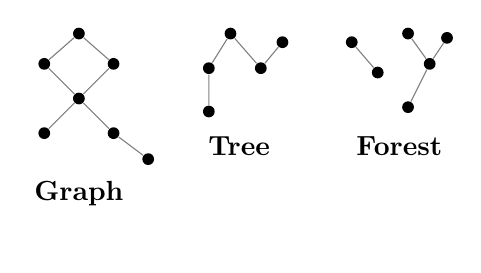
\begin{tikzpicture}[scale=0.55, every node/.style={circle, fill, inner sep=1.5pt}]
    % Graph
    \node (g1) at (0,1.5) {};
    \node (g2) at (-0.8,0.8) {};
    \node (g3) at (0.8,0.8) {};
    \node (g4) at (0,0) {};
    \node (g5) at (-0.8,-0.8) {};
    \node (g6) at (0.8,-0.8) {};
    \node (g7) at (1.6,-1.4) {};
    \draw[gray] (g1) -- (g2) -- (g4) -- (g3) -- (g1);
    \draw[gray] (g4) -- (g5);
    \draw[gray] (g4) -- (g6) -- (g7);
    \node[fill=none] at (0,-2.2) {\textbf{Graph}};

    % Tree
    \node (t1) at (3.5,1.5) {};
    \node (t2) at (3,0.7) {};
    \node (t3) at (4.2,0.7) {};
    \node (t4) at (3,-0.3) {};
    \node (t5) at (4.7,1.3) {};
    \draw[gray] (t1) -- (t2);
    \draw[gray] (t1) -- (t3);
    \draw[gray] (t2) -- (t4);
    \draw[gray] (t3) -- (t5);
    \node[fill=none] at (3.7,-1.1) {\textbf{Tree}};

    % Forest
    \node (f1) at (6.3,1.3) {};
    \node (f2) at (6.9,0.6) {};
    \node (f3) at (7.6,1.5) {};
    \node (f4) at (8.1,0.8) {};
    \node (f5) at (8.5,1.4) {};
    \node (f6) at (7.6,-0.2) {};
    \draw[gray] (f1) -- (f2);
    \draw[gray] (f3) -- (f4);
    \draw[gray] (f4) -- (f5);
    \draw[gray] (f4) -- (f6);
    \node[fill=none] at (7.4,-1.1) {\textbf{Forest}};
\end{tikzpicture}
\end{center}

\begin{definition}[Terminal and Internal Vertices]
    Let $T$ be a tree. If $T$ has only one or two vertices, then each is called a \textbf{terminal vertex} (or leaf). If $T$ has at least three vertices, then a vertex of degree 1 in $T$ is called a terminal vertex, and a vertex of degree $> 1$ in $T$ is called an \textbf{internal vertex}.
\end{definition}

\subsection{Rooted Trees and Binary Trees}

\begin{definition}[Rooted Tree, Level, Height]
    A \textbf{rooted tree} is a tree in which there is one vertex that is distinguished from the others and is called the \textbf{root}.
    
    The \textbf{level} of a vertex is the number of edges along the unique path between it and the root.
\end{definition}

\begin{definition}[Height]
    The \textbf{height} of a rooted tree is the maximum level of any vertex of the tree.
\end{definition}

\begin{definition}[Child, Parent, Sibling, Ancestor, Descendant]
    Given the root or any internal vertex $v$ of a rooted tree, the \textbf{children} of $v$ are all those vertices that are adjacent to $v$ and are one level farther away from the root than $v$. 
    
    If $w$ is a child of $v$, then $v$ is called the \textbf{parent} of $w$, and two distinct vertices that are both children of the same parent are called \textbf{siblings}. 
    
    Given two distinct vertices $v$ and $w$, if $v$ lies on the unique path between $w$ and the root, then $v$ is an \textbf{ancestor} of $w$, and $w$ is a \textbf{descendant} of $v$.
\end{definition}

\vspace{1em}
\begin{center}
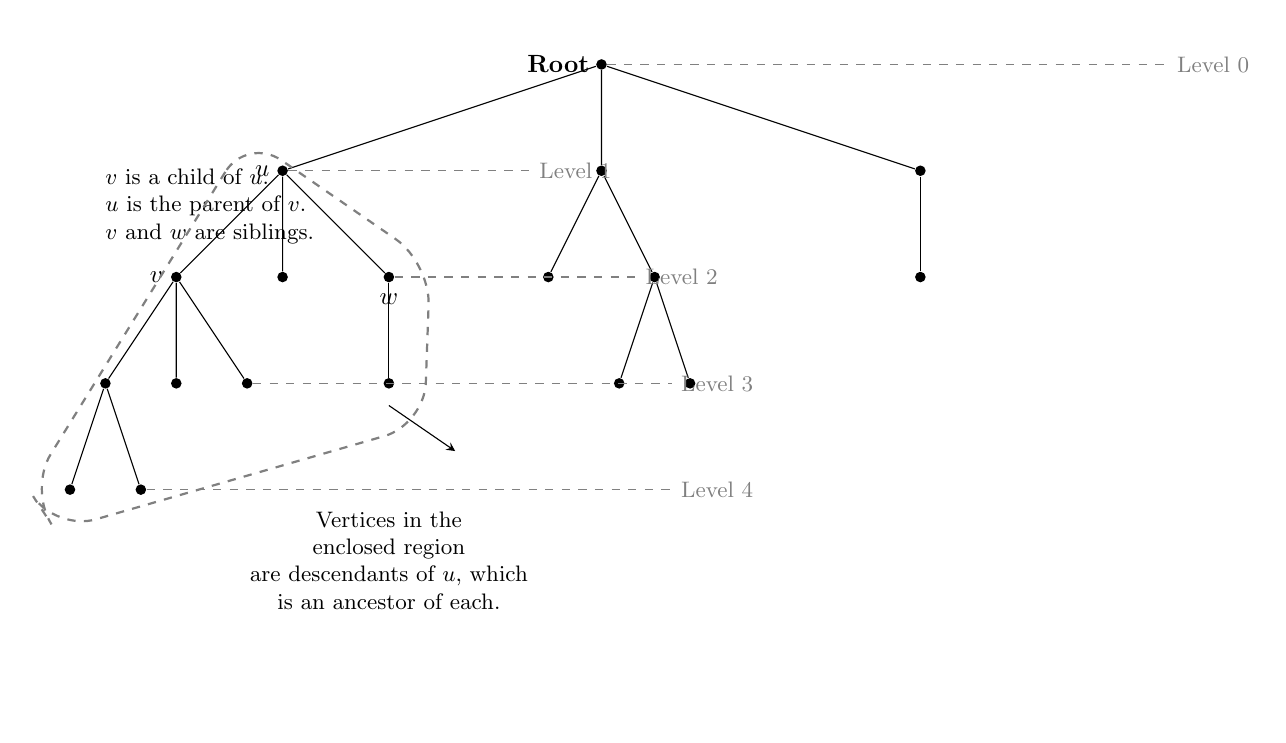
\begin{tikzpicture}[
    scale=0.9, transform shape,
    every node/.style={circle, fill, inner sep=1.5pt},
    level distance=1.5cm,
    level 1/.style={sibling distance=4.5cm},
    level 2/.style={sibling distance=1.5cm},
    level 3/.style={sibling distance=1cm},
    level 4/.style={sibling distance=1cm},
    >=stealth
]

% Draw the tree structure
\node[label=left:{\textbf{Root}}] (root) {}
    child {node[label=left:{$u$}] (u) {}
        child {node[label=left:{$v$}] (v) {}
            child {node (v1) {}
                child {node (v11) {}}
                child {node (v12) {}}
            }
            child {node (v2) {}}
            child {node (v3) {}}
        }
        child {node (um) {}}
        child {node[label=below:{$w$}] (w) {}
            child {node (w1) {}}
        }
    }
    child {node (m) {}
        child {node (m1) {}}
        child {node (m2) {}
            child {node (m21) {}}
            child {node (m22) {}}
        }
    }
    child {node (r) {}
        child {node (r1) {}}
    };

% Draw horizontal level indicators
\begin{scope}[every node/.style={fill=none, right, font=\small}, dashed, gray, thin]
    \draw (root) -- ++(8,0) node {Level 0};
    \draw (u) -- ++(3.5,0) node {Level 1};
    \draw (w) -- ++(3.5,0) node {Level 2};
    \draw (v3) -- ++(6,0) node {Level 3};
    \draw (v12) -- ++(7.5,0) node {Level 4};
\end{scope}

% Text annotations on the left
\node[fill=none, text width=4cm, align=left, font=\small] at (-5, -2) 
    {$v$ is a child of $u$. \\ $u$ is the parent of $v$. \\ $v$ and $w$ are siblings.};

% Dashed boundary for descendants of u
\draw[dashed, thick, gray, rounded corners=15pt] 
    ($(u.north)+(-0.5,0.4)$) -- 
    ($(v11.west)+(-0.5,0)$) -- 
    ($(v11.south)+(-0.2,-0.5)$) -- 
    ($(w1.south)+(0.5,-0.5)$) -- 
    ($(w.east)+(0.5,0.2)$) -- 
    cycle;

% Text annotation for the descendant blob
\node[fill=none, text width=4cm, align=center, font=\small] (descNote) at (-3, -7) 
    {Vertices in the enclosed region \\ are descendants of $u$, which \\ is an ancestor of each.};
\draw[->, shorten >= 2pt] (descNote.north) -- (-2, -5.5);

\end{tikzpicture}
\vspace{0.5em}

\textbf{Figure 10.6.1} A Rooted Tree
\end{center}
\vspace{1em}

\begin{definition}[Binary Tree / Full Binary Tree]
    A \textbf{binary tree} is a rooted tree in which every parent has at most two children. Each child is designated either a left child or a right child (but not both), and every parent has at most one left child and one right child. 
    
    A \textbf{full binary tree} is a binary tree in which each parent has exactly two children.
\end{definition}

\vspace{1em}
\begin{center}
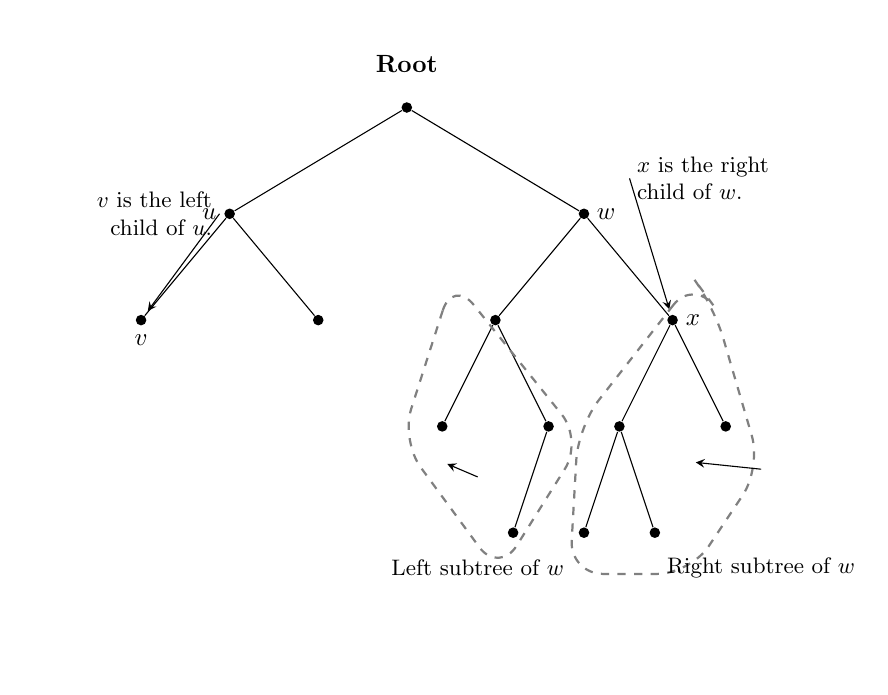
\begin{tikzpicture}[
    scale=0.9, transform shape,
    every node/.style={circle, fill, inner sep=1.5pt},
    level distance=1.5cm,
    level 1/.style={sibling distance=5cm},
    level 2/.style={sibling distance=2.5cm},
    level 3/.style={sibling distance=1.5cm},
    level 4/.style={sibling distance=1cm},
    >=stealth
]

% Draw the tree structure
\node[label=above:{\textbf{Root}}] (root) {}
    child {node[label=left:{$u$}] (u) {}
        child {node[label=below:{$v$}] (v) {}}
        child {node {}}
    }
    child {node[label=right:{$w$}] (w) {}
        child {node (wL) {}
            child {node (wLL) {}}
            child {node (wLR) {}
                child {node (wLRL) {}}
                child[missing] % Forces binary visual layout
            }
        }
        child {node[label=right:{$x$}] (x) {}
            child {node (xL) {}
                child {node (xLL) {}}
                child {node (xLR) {}}
            }
            child {node (xR) {}}
        }
    };

% Annotations for children
\node[fill=none, font=\small, text width=2.5cm, align=right] (vNote) at (-4, -1.5) {$v$ is the left \\ child of $u$.};
\draw[->, shorten >= 2pt] (vNote.east) -- (v);

\node[fill=none, font=\small, text width=2.5cm, align=left] (xNote) at (4.5, -1) {$x$ is the right \\ child of $w$.};
\draw[->, shorten >= 2pt] (xNote.west) -- (x);

% Dashed boundary for Left Subtree of w
\draw[dashed, thick, gray, rounded corners=12pt] 
    ($(wL.north)+(-0.6,0.5)$) -- 
    ($(wLL.west)+(-0.5,-0.2)$) -- 
    ($(wLRL.south)+(-0.2,-0.5)$) -- 
    ($(wLR.east)+(0.4,-0.2)$) -- 
    cycle;
\node[fill=none, font=\small] (Lsub) at (1, -6.5) {Left subtree of $w$};
\draw[->, shorten >= 2pt] (Lsub.north) -- (0.5, -5);

% Dashed boundary for Right Subtree of w
\draw[dashed, thick, gray, rounded corners=12pt] 
    ($(x.north)+(0.3,0.5)$) -- 
    ($(xL.west)+(-0.5,0)$) -- 
    ($(xLL.south)+(-0.2,-0.5)$) -- 
    ($(xLR.south)+(0.5,-0.5)$) -- 
    ($(xR.south)+(0.5,-0.5)$) --
    ($(x.east)+(0.5,0.2)$) -- 
    cycle;
\node[fill=none, font=\small] (Rsub) at (5, -6.5) {Right subtree of $w$};
\draw[->, shorten >= 2pt] (Rsub.north) -- (4, -5);

\end{tikzpicture}
\vspace{0.5em}

\textbf{Figure 10.6.2} A Binary Tree
\end{center}
\vspace{1em}

\begin{definition}[Left Subtree / Right Subtree]
    Given any parent $v$ in a binary tree $T$, if $v$ has a left child, then the \textbf{left subtree} of $v$ is the binary tree whose root is the left child of $v$, whose vertices consist of the left child of $v$ and all its descendants, and whose edges consist of all those edges of $T$ that connect the vertices of the left subtree. The \textbf{right subtree} of $v$ is defined analogously.
\end{definition}

\subsection{Tree Traversal}

\textbf{Tree traversal} (also known as tree search) is the process of visiting each node in a tree data structure exactly once in a systematic manner. There are two main types of traversal: breadth-first search (BFS) and depth-first search (DFS).
\begin{itemize}
    \item In \textbf{BFS}, it starts at the root and visits its adjacent vertices, and then moves to the next level.
    \item In \textbf{DFS}, it starts at the root node and explores as far as possible along each branch before backtracking.
\end{itemize}

\subsubsection*{Depth-First Search (DFS) Traversal Types}
There are three types of depth-first traversal:
\begin{enumerate}
    \item \textbf{Pre-order:} Current $\rightarrow$ Left $\rightarrow$ Right
    \item \textbf{In-order:} Left $\rightarrow$ Current $\rightarrow$ Right
    \item \textbf{Post-order:} Left $\rightarrow$ Right $\rightarrow$ Current
\end{enumerate}

\begin{note}[Tips for Tracing]
    \textbf{Tip 1:} Draw `dots' on the side of the nodes, which represent the order in which they are searched/visited:
    \begin{itemize}
        \item For \textbf{pre-order}: dot on the \textbf{left} of each node.
        \item For \textbf{in-order}: dot \textbf{below} each node.
        \item For \textbf{post-order}: dot to the \textbf{right} of each node.
    \end{itemize}
    \textbf{Tip 2:} For pre-order traversal, the root is at the start. For post-order, the root is at the end. For in-order traversal, the root is in the middle of the sequence, and all nodes to the left of the root are the left children and all nodes to the right of the root are the right children.
\end{note}

\vspace{1em}
\begin{center}
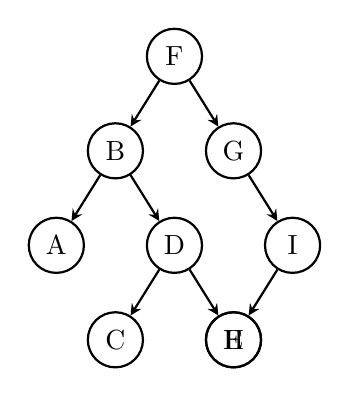
\begin{tikzpicture}[
    every node/.style={circle, draw, thick, minimum size=0.7cm, inner sep=0pt},
    level distance=1.2cm,
    edge from parent/.style={draw, thick, ->, >=stealth}
]
    % DFS Tree
    \node (F) at (0,0) {F}
        child {node (B) {B}
            child {node (A) {A}}
            child {node (D) {D}
                child {node (C) {C}}
                child {node (E) {E}}
            }
        }
        child {node (G) {G}
            child[missing] % Keeps G's child strictly to the right visually
            child {node (I) {I}
                child {node (H) {H}}
                child[missing]
            }
        };
\end{tikzpicture}
\end{center}
\begin{center}
\textbf{Figure 1: DFS Traversal} \\
\vspace{0.5em}
\begin{tabular}{rl}
    \textbf{Pre-order:} & F, B, A, D, C, E, G, I, H \\
    \textbf{In-order:} & A, B, C, D, E, F, G, H, I \\
    \textbf{Post-order:} & A, C, E, D, B, H, I, G, F
\end{tabular}
\end{center}
\vspace{1em}

\begin{center}
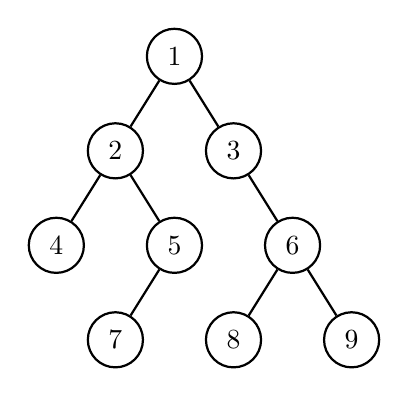
\begin{tikzpicture}[
    every node/.style={circle, draw, thick, minimum size=0.7cm, inner sep=0pt},
    level distance=1.2cm,
    edge from parent/.style={draw, thick, -}
]
    % BFS Tree
    \node (1) at (0,0) {1}
        child {node (2) {2}
            child {node (4) {4}}
            child {node (5) {5}
                child {node (7) {7}}
                child[missing]
            }
        }
        child {node (3) {3}
            child[missing]
            child {node (6) {6}
                child {node (8) {8}}
                child {node (9) {9}}
            }
        };
\end{tikzpicture}
\end{center}
\begin{center}
\textbf{Figure 2: BFS Traversal}
\end{center}
\vspace{1em}

\subsection{Spanning Trees and Shortest Paths}

\begin{definition}[Spanning Tree]
    A \textbf{spanning tree} for a graph $G$ is a subgraph of $G$ that contains every vertex of $G$ and is a tree. \\
    *(Spanning tree = remove edges from the graph until you cannot remove any more edges without disconnecting the graph).*
\end{definition}

\begin{definition}[Weighted Graph]
    A \textbf{weighted graph} is a graph for which each edge has an associated positive real number weight. The sum of the weights of all the edges is the total weight of the graph.
\end{definition}

\begin{definition}[Minimum Spanning Tree (MST)]
    A \textbf{minimum spanning tree} for a connected weighted graph is a spanning tree that has the least possible total weight compared to all other spanning trees for the graph. 
    
    If $G$ is a weighted graph and $e$ is an edge of $G$, then $w(e)$ denotes the weight of $e$ and $w(G)$ denotes the total weight of $G$.
\end{definition}

\subsubsection*{Kruskal's Algorithm for MST}
\textbf{Input:} $G$, a connected weighted graph.
\begin{enumerate}[label=\arabic*.]
    \item Initialize $T$ to have all the vertices of $G$ and no edges.
    \item Let $E$ be the set of all edges of $G$, and let $m = 0$.
    \item While $(m < n - 1)$:
    \begin{enumerate}[label=(\alph*)]
        \item Find an edge $e$ in $E$ of least weight.
        \item Delete $e$ from $E$.
        \item If the addition of $e$ to the edge set of $T$ does not produce a circuit, then add $e$ to the edge set of $T$ and set $m = m + 1$.
    \end{enumerate}
    \item \textbf{Output:} $T$ [$T$ is a minimum spanning tree for $G$].
\end{enumerate}

\subsubsection*{Prim's Algorithm for MST}
\textbf{Input:} $G$, a connected weighted graph with $n$ vertices.
\begin{enumerate}[label=\arabic*.]
    \item Pick a vertex $v$ of $G$ and let $T$ be the graph with this vertex only.
    \item Let $V$ be the set of all vertices of $G$ except $v$.
    \item For $i = 1$ to $n - 1$:
    \begin{enumerate}[label=(\alph*)]
        \item Find an edge $e$ of $G$ such that (1) $e$ connects $T$ to one of the vertices in $V$, and (2) $e$ has the least weight of all edges connecting $T$ to a vertex in $V$. Let $w$ be the endpoint of $e$ that is in $V$.
        \item Add $e$ and $w$ to the edge and vertex sets of $T$, and delete $w$ from $V$.
    \end{enumerate}
    \item \textbf{Output:} $T$ [$T$ is a minimum spanning tree for $G$].
\end{enumerate}

\subsubsection*{Dijkstra's Algorithm for Shortest Path}
\begin{enumerate}[label=\arabic*.]
    \item Let $v$ be the initial node (the source). The distance of a node $w$ is defined as the distance from the initial node $v$.
    \item Set the distances of all nodes to be infinity (except $v$), and mark all nodes as unvisited (including $v$). Set the distance of the initial node to itself as 0.
    \item Loop: while there are still unvisited nodes,
    \begin{enumerate}[label=(\alph*)]
        \item Pick the vertex with the smallest distance to the initial node $v$ as the current node $u$.
        \item Mark $u$ as visited.
        \item For each adjacent (neighbouring) node $n$ of the current node that is unvisited, compare the current distance of $n$ with the distance obtained from traversing from $u$ to $n$, i.e. $\text{distance}(u) + \text{weight}(u,n)$. Take the smaller of the two and set it as the new distance of $n$.
        \item If there are still unvisited nodes, repeat from step 3.
    \end{enumerate}
    \item Return the distance of the target (destination) node from the initial node $v$.
\end{enumerate}
\begin{note}
    There are many variations of Dijkstra's Algorithm; some can return you the exact path taken. This version only returns the shortest distance of the target from the source node, but they are all similar in essence.
\end{note}

\section{Matrices (Continued)}

\begin{theorem}[10.3.2: Powers of an Adjacency Matrix]
    If $G$ is a graph with vertices $v_1, v_2, \dots, v_m$ and $\mathbf{A}$ is the adjacency matrix of $G$, then for each positive integer $n$ and for all integers $i, j = 1, 2, \dots, m$:
    \begin{center}
        The $ij$-th entry of $\mathbf{A}^n =$ the number of walks of length $n$ from $v_i$ to $v_j$.
    \end{center}
    *(Note: $\mathbf{A}^0$ is the identity matrix $\mathbf{I}$.)*
\end{theorem}

\section{Graph Theory (Continued)}

\begin{theorem}[10.4.1: Graph Isomorphism is an Equivalence Relation]
    Let $S$ be a set of graphs and let $\cong$ be the relation of graph isomorphism on $S$. Then $\cong$ is an equivalence relation on $S$.
\end{theorem}

\subsection{Euler's Formula}
For a connected planar simple graph $G = (V,E)$ with $e = |E|$ and $v = |V|$, if we let $f$ be the number of faces, then:
\[ f = e - v + 2 \]

\begin{center}
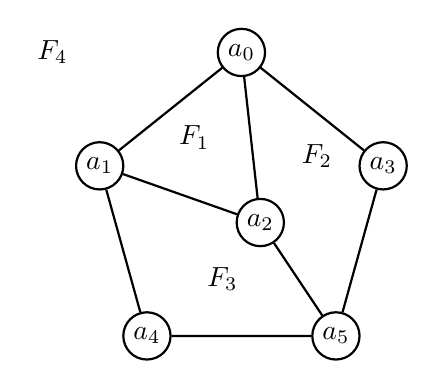
\begin{tikzpicture}[
    scale=1.2, 
    every node/.style={circle, draw, thick, fill=white, inner sep=1.5pt, minimum size=6mm}
]
    % Nodes
    \node (a0) at (0, 2) {$a_0$};
    \node (a1) at (-1.5, 0.8) {$a_1$};
    \node (a4) at (-1, -1) {$a_4$};
    \node (a5) at (1, -1) {$a_5$};
    \node (a3) at (1.5, 0.8) {$a_3$};
    \node (a2) at (0.2, 0.2) {$a_2$};

    % Edges (Outer)
    \draw[thick] (a0) -- (a1) -- (a4) -- (a5) -- (a3) -- (a0);
    
    % Edges (Inner)
    \draw[thick] (a0) -- (a2);
    \draw[thick] (a1) -- (a2);
    \draw[thick] (a5) -- (a2);

    % Face Labels (No circles for these)
    \node[draw=none, fill=none] at (-0.5, 1.1) {$F_1$};
    \node[draw=none, fill=none] at (0.8, 0.9) {$F_2$};
    \node[draw=none, fill=none] at (-0.2, -0.4) {$F_3$};
    \node[draw=none, fill=none] at (-2, 2) {$F_4$};
\end{tikzpicture}

\vspace{0.5em}
$e=8, \quad v=6 \quad \Rightarrow \quad f = 8 - 6 + 2 = 4$
\end{center}

\subsection{Graph Examples: Hamiltonian vs. Non-Hamiltonian}

\begin{center}
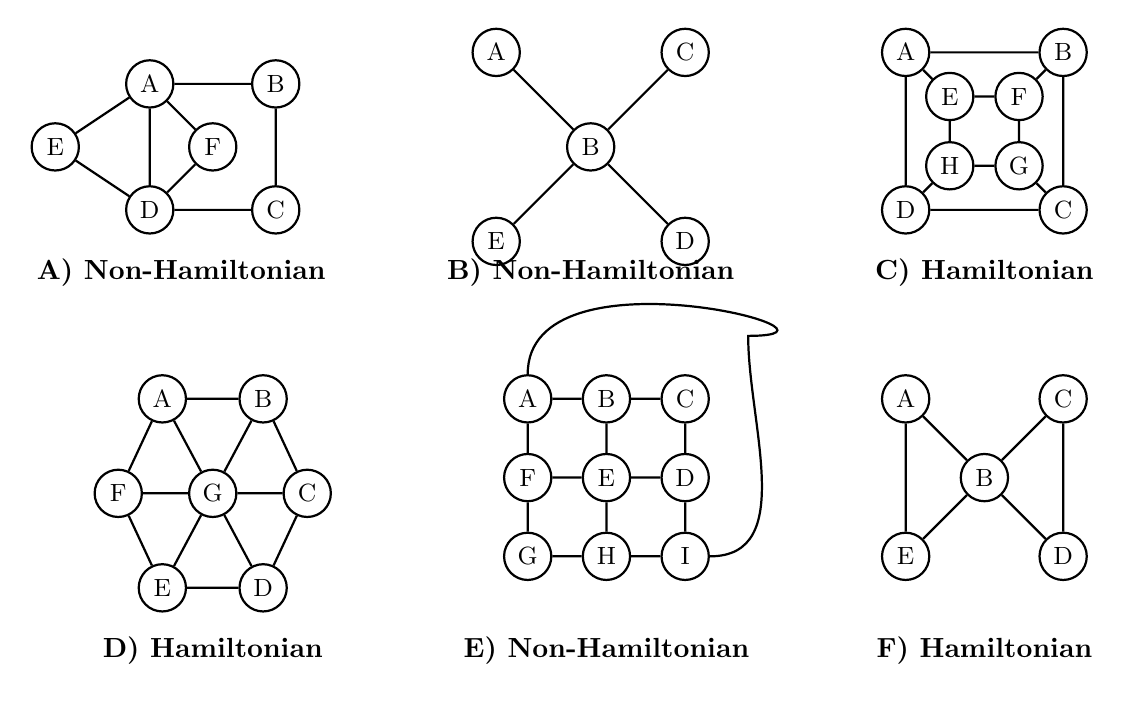
\begin{tikzpicture}[
    scale=0.8,
    dot/.style={circle, fill=white, draw=black, thick, inner sep=2pt, minimum size=6mm},
    font=\small
]
    % --- GRAPH A (Non-Hamiltonian) ---
    \begin{scope}[xshift=0cm, yshift=0cm]
        \node[dot] (A) at (0, 2) {A};
        \node[dot] (B) at (2, 2) {B};
        \node[dot] (C) at (2, 0) {C};
        \node[dot] (D) at (0, 0) {D};
        \node[dot] (E) at (-1.5, 1) {E};
        \node[dot] (F) at (1, 1) {F};
        
        \draw[thick] (A)--(B)--(C)--(D)--(A);
        \draw[thick] (E)--(A) (E)--(D);
        \draw[thick] (F)--(A) (F)--(D);
        \node[draw=none, fill=none, font=\bfseries] at (0.5, -1) {A) Non-Hamiltonian};
    \end{scope}

    % --- GRAPH B (Non-Hamiltonian) ---
    \begin{scope}[xshift=6cm, yshift=0cm]
        \node[dot] (B) at (1, 1) {B};
        \node[dot] (A) at (-0.5, 2.5) {A};
        \node[dot] (C) at (2.5, 2.5) {C};
        \node[dot] (E) at (-0.5, -0.5) {E};
        \node[dot] (D) at (2.5, -0.5) {D};
        
        \draw[thick] (A)--(B) (C)--(B) (E)--(B) (D)--(B);
        \node[draw=none, fill=none, font=\bfseries] at (1, -1) {B) Non-Hamiltonian};
    \end{scope}

    % --- GRAPH C (Hamiltonian) ---
    \begin{scope}[xshift=12cm, yshift=0cm]
        \node[dot] (A) at (0, 2.5) {A};
        \node[dot] (B) at (2.5, 2.5) {B};
        \node[dot] (C) at (2.5, 0) {C};
        \node[dot] (D) at (0, 0) {D};
        \node[dot] (E) at (0.7, 1.8) {E};
        \node[dot] (F) at (1.8, 1.8) {F};
        \node[dot] (G) at (1.8, 0.7) {G};
        \node[dot] (H) at (0.7, 0.7) {H};
        
        \draw[thick] (A)--(B)--(C)--(D)--(A);
        \draw[thick] (E)--(F)--(G)--(H)--(E);
        \draw[thick] (A)--(E) (B)--(F) (C)--(G) (D)--(H);
        \node[draw=none, fill=none, font=\bfseries] at (1.25, -1) {C) Hamiltonian};
    \end{scope}

    % --- GRAPH D (Hamiltonian) ---
    \begin{scope}[xshift=0cm, yshift=-5.5cm]
        \node[dot] (G) at (1, 1) {G};
        \node[dot] (A) at (0.2, 2.5) {A};
        \node[dot] (B) at (1.8, 2.5) {B};
        \node[dot] (C) at (2.5, 1) {C};
        \node[dot] (D) at (1.8, -0.5) {D};
        \node[dot] (E) at (0.2, -0.5) {E};
        \node[dot] (F) at (-0.5, 1) {F};
        
        \draw[thick] (A)--(B)--(C)--(D)--(E)--(F)--(A);
        \draw[thick] (A)--(G) (B)--(G) (C)--(G) (D)--(G) (E)--(G) (F)--(G);
        \node[draw=none, fill=none, font=\bfseries] at (1, -1.5) {D) Hamiltonian};
    \end{scope}

    % --- GRAPH E (Non-Hamiltonian) ---
    \begin{scope}[xshift=6cm, yshift=-5.5cm]
        \node[dot] (A) at (0, 2.5) {A};
        \node[dot] (B) at (1.25, 2.5) {B};
        \node[dot] (C) at (2.5, 2.5) {C};
        \node[dot] (F) at (0, 1.25) {F};
        \node[dot] (E) at (1.25, 1.25) {E};
        \node[dot] (D) at (2.5, 1.25) {D};
        \node[dot] (G) at (0, 0) {G};
        \node[dot] (H) at (1.25, 0) {H};
        \node[dot] (I) at (2.5, 0) {I};
        
        \draw[thick] (A)--(B)--(C) (F)--(E)--(D) (G)--(H)--(I);
        \draw[thick] (A)--(F)--(G) (B)--(E)--(H) (C)--(D)--(I);
        % Curved edge from A to I
        \draw[thick] (A) to[out=90, in=0, looseness=1.5] (3.5, 3.5) to[out=270, in=0, looseness=1] (I);
        \node[draw=none, fill=none, font=\bfseries] at (1.25, -1.5) {E) Non-Hamiltonian};
    \end{scope}

    % --- GRAPH F (Hamiltonian) ---
    \begin{scope}[xshift=12cm, yshift=-5.5cm]
        \node[dot] (B) at (1.25, 1.25) {B};
        \node[dot] (A) at (0, 2.5) {A};
        \node[dot] (E) at (0, 0) {E};
        \node[dot] (C) at (2.5, 2.5) {C};
        \node[dot] (D) at (2.5, 0) {D};
        
        \draw[thick] (A)--(E)--(B)--(A);
        \draw[thick] (C)--(D)--(B)--(C);
        \node[draw=none, fill=none, font=\bfseries] at (1.25, -1.5) {F) Hamiltonian};
    \end{scope}
\end{tikzpicture}
\end{center}

\section{Trees (Continued)}

\begin{lemma}[10.5.1]
    Any non-trivial tree has at least one vertex of degree 1.
\end{lemma}

\begin{theorem}[10.5.2]
    Any tree with $n$ vertices ($n > 0$) has $n - 1$ edges.
\end{theorem}

\begin{lemma}[10.5.3]
    If $G$ is any connected graph, $C$ is any circuit in $G$, and one of the edges of $C$ is removed from $G$, then the graph that remains is still connected.
\end{lemma}

\begin{theorem}[10.5.4]
    If $G$ is a connected graph with $n$ vertices and $n - 1$ edges, then $G$ is a tree.
\end{theorem}

\begin{lemma}[10.5.5]
    Let $G$ be a simple, undirected graph. If there are two distinct paths from a vertex $v$ to a different vertex $w$, then $G$ contains a cycle (and hence $G$ is cyclic).
    \\ *(i.e., 2 distinct paths $\Rightarrow G$ is cyclic. By contrapositive: $G$ is acyclic $\Rightarrow$ at most one distinct path between any $v, w$).*
\end{lemma}

\begin{theorem}[10.6.1: Full Binary Tree Theorem]
    If $T$ is a full binary tree with $k$ internal vertices, then $T$ has a total of $2k + 1$ vertices and has $k + 1$ terminal vertices (leaves).
\end{theorem}

\begin{theorem}[10.6.2: Height of a Binary Tree]
    For non-negative integers $h$, if $T$ is any binary tree with height $h$ and $t$ terminal vertices (leaves), then:
    \[ t \leq 2^h \quad \text{or equivalently,} \quad \log_2(t) \leq h \]
\end{theorem}

\begin{proposition}[10.7.1]
    \hfill
    \begin{enumerate}
        \item Every connected graph has a spanning tree.
        \item Any two spanning trees for a graph have the same number of edges.
    \end{enumerate}
\end{proposition}

\section{Summary of Graph Proofs (Tutorial 11)}

\begin{itemize}
    \item \textbf{Min/Max Edges of a Connected Graph (Q1):} For a simple connected graph with $n$ ($n > 0$) vertices, there are a minimum of $(n-1)$ edges and a maximum of $\frac{n(n-1)}{2}$ edges.
    \begin{itemize}
        \item \textit{Proof concept:} Since it's connected, the minimum is $n-1$ (a spanning tree). The maximum is derived from the Handshake theorem for a complete graph, which sums the AP series $1 + 2 + \dots + (n-1)$.
    \end{itemize}
    \item \textbf{Number of Simple Graphs (Q2):} For a graph with $n$ ($n > 1$) vertices, there are $2^{\binom{n}{2}}$ possible simple graphs.
    \begin{itemize}
        \item \textit{Proof concept:} There are a maximum of $\binom{n}{2}$ possible edges. For each edge, you can either include it or not include it (2 choices), so the permutations are $2$ to the power of the max number of edges.
    \end{itemize}
    \item \textbf{Planar Bounds (Q2):} For any planar graph with $f$ faces, $v$ vertices, and $e$ edges:
    \begin{enumerate}[label=(\alph*)]
        \item $3f \leq 2e$: Each face must have at least 3 edges, and each edge can be counted at most 2 times (borders between 2 faces).
        \item $e \leq 3v - 6$: Derived algebraically by substituting the first inequality into Euler's formula ($f = e - v + 2$).
    \end{enumerate}
    \item \textbf{Edges in Connected vs Acyclic (Q5/Q6):} Let $G = (V,E)$ be a simple, undirected graph.
    \begin{itemize}
        \item If $G$ is connected, then $|E| \geq |V| - 1$.
        \item If $G$ is acyclic, then $|E| \leq |V| - 1$.
    \end{itemize}
    \item \textbf{Tree Path Uniqueness (Q7):} Let $G = (V,E)$ be a simple, undirected graph. $G$ is a tree \textbf{iff} there is exactly one path between every pair of vertices.
\end{itemize}

\end{document}